\documentclass[conference]{IEEEtran}
\IEEEoverridecommandlockouts
\usepackage{cite}
\usepackage{amsmath,amssymb}
\usepackage{graphicx}
\usepackage{booktabs}
\usepackage{array}
\usepackage{tabularx}
\usepackage{xcolor}
\usepackage{listings}
\usepackage{tikz}
\usetikzlibrary{arrows.meta,positioning,fit,calc,shapes.geometric}
\usepackage{balance}
\usepackage[hidelinks]{hyperref}

\newcommand{\thinunit}[2]{#1\,#2}

\lstset{basicstyle=\ttfamily\scriptsize,breaklines=true,breakatwhitespace=false,
  columns=fullflexible,frame=single,xleftmargin=0pt,framexleftmargin=0pt,
  showstringspaces=false,aboveskip=4pt,belowskip=4pt}

\def\BibTeX{{\rm B\kern-.05em{\sc i\kern-.025em b}\kern-.08em T\kern-.1667em\lower.7ex\hbox{E}\kern-.125emX}}

\begin{document}

\title{Quantx: An NSE Equity Paper-Trading Workspace with Boundary-Enforced Market Data, Depth-Based Local Order Matching, and Transactional SafePoint Recovery}

\author{\IEEEauthorblockN{Bhavik Achotani}
\IEEEauthorblockA{Department of Information Technology\\
Thadomal Shahani Engineering College, University of Mumbai\\
Mumbai, India\\
achotanibhavikoffice@gmail.com}}

\maketitle

\begin{abstract}
In this work, we developed Quantx, an exchange-style paper-trading workspace for National Stock Exchange of India (NSE) equities in which simulated orders are matched locally against streamed market depth and protected by transactional state snapshots. The system is organized as four tiers: a React client, a FastAPI service tier, an in-process market-data decoding and matching tier, and a PostgreSQL ledger paired with a Redis quote cache. Its foundational design principle is a strict architectural boundary between a market-data plane, which may only read authentication, instrument, and quote data from upstream providers, and an accounting plane, which alone creates orders, fills, statutory charges, cash movements, positions, and recovery snapshots; paper orders are never routed to an external broker or exchange order interface. Inside this boundary, the system normalizes prices to tick size, validates circuit, board-lot, and freeze constraints, walks five-level bid and ask depth with partial fills, applies product-aware brokerage and Indian statutory charges, discards duplicate and older-timestamp packets, refuses market orders when depth is stale, and provides atomic SafePoint state rollback alongside non-destructive multi-modal What-If stress testing and a guardrailed non-advisory learning guide. We evaluated the integrated workflow against a last-price, zero-charge, arrival-order baseline (B0) across $N=50$ scripted orders spanning Typical ($N_1=20$), Boundary ($N_2=20$), and Adversarial ($N_3=10$ valid orders plus $N_{\mathrm{adv}}=50$ injected fault events) scenario profiles on a live PostgreSQL 16.15 and Redis 7.4.11 stack. Quantx achieved zero ledger-reconciliation error ($\text{mean}=\thinunit{0.00}{INR}$, $\text{max}=\thinunit{0.00}{INR}$ vs.\ B0 $\text{mean}=\thinunit{19{,}684.41}{INR}$, $\text{max}=\thinunit{227{,}398.32}{INR}$), zero fill-price deviation ($\thinunit{0.00}{INR/share}$ vs.\ B0 $\thinunit{1.60}{INR/share}$ across $N_f=73$ fills), zero charge deviation ($\thinunit{0.00}{INR/fill}$ vs.\ B0 $\thinunit{33.08}{INR/fill}$), and zero adversarial fault leaks across all 50 injected disorder, staleness, idempotency, and rule-violation events, while maintaining sub-millisecond quote ingestion ($\text{p99}=\thinunit{0.06}{ms}$) and sub-\thinunit{120}{ms} five-level match-and-commit latency ($\text{p50}=\thinunit{71.02}{ms}$, $\text{p99}=\thinunit{118.02}{ms}$). These results support the engineering feasibility of boundary-enforced local paper execution for NSE equity practice; they do not establish fidelity to live exchange queue priority, educational learning outcomes, or production brokerage readiness.
\end{abstract}

\begin{IEEEkeywords}
Paper Trading, Order Matching, Limit Order Book, Market Depth, Indian Equities, Transaction Charges, Idempotent Submission, Out-of-Order Market Data, SafePoint State Recovery, Financial Education Software.
\end{IEEEkeywords}

\section{Introduction}

Software that enables a learner to practice securities trading must reconcile two classes of information whose ground truth is owned by distinct parties. The first class is market data: instrument reference masters, top-of-book quotes, and multi-level order-book depth that originate at an exchange or its licensed vendor, arrive as an asynchronous, high-rate stream, and cannot be altered by the client application \cite{harris2003,hasbrouck2007,gould2013}. The second class is account state: orders, partial fills, statutory charges, cash balances, positions, and recovery checkpoints that exist solely because the application records them, and whose internal consistency the application must guarantee through atomic transactional storage \cite{gray1993,kleppmann2017}. A practice environment is trustworthy only when the first class of information is treated strictly as read-only input and the second as an authoritative, auditable ledger.

Unconstrained retail trading simulators typically blur this separation and exhibit three recurring failure modes:
\begin{itemize}
  \item \textbf{Fill-Model Fragility:} Filling an order of arbitrary size at the last traded price ignores finite displayed liquidity at each price level and the bid--ask spread, even though empirical execution prices depend directly on how far an order walks the limit order book and on order quantity \cite{almgren2001,kyle1985,glosten1985,cont2010}.
  \item \textbf{Charge and Product-Rule Blindness:} Transaction costs and portfolio turnover are primary determinants of individual investors' net returns \cite{barber2000,barber2002,barber2009}. In Indian cash equities, statutory charges—Securities Transaction Tax (STT), exchange transaction fees, SEBI turnover fees, stamp duty, and Goods and Services Tax (GST)—differ sharply by product type (Cash and Carry delivery, CNC, versus Margin Intraday Square-off, MIS) and by order side. A simulator that omits per-fill statutory charges or exchange lot/circuit rules reports systematically inflated profit and loss.
  \item \textbf{Feed-Disorder and State-Corruption Fragility:} Real network feeds deliver duplicated, delayed, and out-of-order frames in which processing-time arrival order diverges from exchange event-time order \cite{akidau2015,lamport1978,hasbrouck2013}. A simulator that applies packets in arrival order allows a delayed quote to overwrite a newer book state, and a simulator without transactional state snapshots or non-advisory guardrails leaves learners unable to recover cleanly from accidental over-leveraging or simulated flash-crash exercises.
\end{itemize}

This study evaluates an integrated, boundary-enforced workspace—\textbf{Quantx}—rather than any single mechanism in isolation. The workflow combines server-side-only provider credentials; an architectural provider boundary that excludes order-placement endpoints; big-endian binary frame decoding with paise-to-rupee normalization; event-time ordering and duplicate suppression; a configurable stale-depth guard for market orders; tick rounding and circuit, board-lot, freeze, product, and buying-power validation at admission; conservative cash reservation; idempotent order submission; five-level depth-walking matching with partial fills and Immediate-or-Cancel (IOC) remainder cancellation; product-aware per-fill statutory charges; single-transaction persistence of orders, trades, charge breakdowns, cash-ledger entries, and positions; an immutable order-event audit trail; account-level Market Stress Mode; a transactional SafePoint Recovery Shield with autonomous fault rollback; a multi-modal What-If scenario laboratory; and a dual-mode, SEBI-compliant non-advisory learning guide.

\subsection{Problem Statement}
Existing literature treats these concerns in separate silos: market-microstructure models characterize limit order book dynamics \cite{gould2013,cont2010}, empirical finance studies quantify retail transaction drag \cite{barber2009,sebi2023}, and distributed-systems research formalizes out-of-order stream processing, idempotency, and ACID transactions \cite{akidau2015,helland2012,gray1993}. Applied piecemeal, each leaves critical vulnerabilities at the application boundary. A depth-walking fill model without an integrated statutory charge engine produces drifted cash balances; a charge engine without a stale-depth gate bills executions against frozen market snapshots; and an accounting ledger without an enforced provider boundary risks leaking practice orders to a live brokerage endpoint or leaving learner portfolios wedged after stress experiments.

The research and systems-engineering problem is to design and verify a unified execution architecture for NSE equity practice in which (i) upstream market data is strictly read-only input across a zero-order provider boundary, (ii) every order, partial fill, statutory charge component, cash movement, position update, and state checkpoint is computed and persisted atomically inside the application, and (iii) the ledger remains exact to the paisa under duplicate, out-of-order, bursty, and stale market updates, while explicitly delineating which properties are empirically measured and which remain outside the scope of simulation.

\subsection{Project Objectives}
\begin{itemize}
  \item \textbf{Implement} a local paper-trading execution engine supporting \texttt{MARKET}, \texttt{LIMIT}, Stop-Loss Limit (\texttt{SL}), and Stop-Loss Market (\texttt{SL-M}) orders with five-level partial fills, modification, cancellation, and \texttt{DAY}/\texttt{IOC} validity.
  \item \textbf{Enforce} an authenticated market-data plane behind a strict provider boundary that permits authentication, instrument-master synchronization, and quote streaming only.
  \item \textbf{Construct} an ACID transactional accounting plane that persists per-level fills, six-component Indian statutory charges, double-tagged cash-ledger entries, signed positions, and atomic SafePoint state snapshots.
  \item \textbf{Develop} deterministic feed-disorder filtering, stale-depth market-order gating, non-destructive multi-modal What-If stress analysis, and guardrailed educational assistance.
  \item \textbf{Evaluate} the integrated system against a naive baseline (B0) across Typical, Boundary, and Adversarial profiles on a live PostgreSQL and Redis deployment, reporting full percentile distributions alongside exact reconciliation audits.
\end{itemize}

\subsection{Contributions}
\begin{enumerate}
  \item A four-tier system architecture enforcing a hard separation between the read-only market-data plane and the transactional accounting and resilience plane (Sections~III and~IV).
  \item A formal mathematical specification of five-level depth-walking order matching, conservative buying-power reservation, product-aware Indian statutory charges, signed position accounting, SafePoint state diffing and rollback, and multi-modal What-If shock projections, with every variable and unit explicitly defined (Section~V).
  \item A four-phase execution workflow, module configuration registry, validated request contract, and dual-mode guardrailed support architecture (Section~VI).
  \item A reproducible empirical evaluation across $N=50$ scripted orders ($N_f=73$ fills) and $N_{\mathrm{adv}}=50$ adversarial fault injections comparing Quantx against baseline B0, paired with candid validity boundaries and four pre-registered future evaluation protocols (Sections~VII--IX).
\end{enumerate}

The remainder of this paper is structured as follows. Section~II reviews related literature and formulates three falsifiable hypotheses. Section~III presents the four-tier architecture. Sections~IV and~V detail the market-data plane and the matching, charging, recovery, and scenario mechanisms. Section~VI documents runtime configuration, structured validation, and the guardrailed assistant. Section~VII reports the experimental setup and empirical results. Section~VIII discusses architectural limitations, code--documentation discrepancies, and ethical boundaries, and Section~IX concludes with reproducible future protocols.

\section{Related Work}

\subsection{Market Microstructure and Limit Order Book Execution}
Theoretical and empirical market-microstructure research establishes why execution prices depend on displayed order-book liquidity rather than the most recent trade print. Comprehensive surveys of limit order books characterize spread dynamics, depth profiles, and queue priority \cite{gould2013}, while stochastic queueing models demonstrate how top-of-book and multi-level depth govern short-horizon fill probabilities \cite{cont2010}. Optimal execution frameworks link order size and execution horizon to temporary and permanent market impact \cite{almgren2001}, equilibrium models connect adverse selection and order flow to bid--ask spreads \cite{kyle1985,glosten1985}, and empirical studies document how markets digest multi-level liquidity consumption \cite{bouchaud2009,hasbrouck2007,harris2003}. While these works formalize exchange matching and price formation, they do not specify an application-level software architecture that reproduces multi-level depth walking and partial-fill accounting inside an isolated learner workspace while guaranteeing that external market feeds remain strictly read-only.

\subsection{Transaction Costs and Retail Investor Performance}
Empirical studies of individual brokerage accounts consistently show that transaction costs and excessive turnover significantly erode net equity returns \cite{barber2000,barber2002}, producing substantial aggregate wealth transfers from active retail traders \cite{barber2009}. In the Indian market context, a landmark study by the Department of Economic and Policy Analysis (DEPA) of the Securities and Exchange Board of India (SEBI) documented that 89\% of individual traders in the equity futures and options (F\&O) segment incurred net losses, with transaction costs consuming a major share of gross trading turnover \cite{sebi2023}. Although SEBI's empirical report focused on derivatives rather than the cash-equity segment studied here, its findings underscore the pedagogical necessity of modeling product-specific brokerage, STT, stamp duty, exchange turnover fees, SEBI regulatory fees, and GST on every simulated fill rather than reporting frictionless gross returns.

\subsection{Experiential Learning, Simulation Fidelity, and Overfitting Risks}
Experiential learning theory emphasizes concrete action and reflective observation in risk-free environments prior to live performance \cite{kolb1984}. In quantitative finance, however, simulated performance carries severe epistemic hazards: Bailey et al.\ \cite{bailey2014} prove that repeated strategy testing on historical or synthetic paths easily generates false discoveries through backtest overfitting. Computational reproducibility standards therefore require that simulation claims be accompanied by exact parameter disclosures, deterministic replay artifacts, and explicit scope boundaries \cite{peng2011,wohlin2012}. Because no controlled human-subject study was conducted in this work, we make zero claims regarding educational efficacy or live trading skill transfer, focusing strictly on systems-level accounting and execution conformance.

\subsection{Event-Time Disorder, Idempotency, and Transactional Recovery}
Distributed stream-processing literature distinguishes event time (when an exchange generates a quote) from processing time (when a downstream server receives it), demonstrating that network jitter and reconnection bursts inevitably cause out-of-order and duplicate arrivals \cite{akidau2015,lamport1978,hasbrouck2013}. Simultaneously, enterprise data-intensive systems rely on client-supplied idempotency keys to render network retries safe \cite{helland2012} and on ACID relational transactions with snapshot recovery to prevent partial state corruption \cite{gray1993,kleppmann2017,fowler2002}. Existing financial simulators rarely integrate event-time quote filtering, stale-depth market-order blocking, idempotent order admission, and user-invocable portfolio SafePoint rollbacks into a single auditable pipeline.

\textbf{Research Gap and Hypotheses.} To our knowledge, no prior peer-reviewed system combines, in one empirically audited workflow, (i) a zero-order provider boundary for NSE equities, (ii) five-level depth-walking partial fills with six-component Indian statutory charges, (iii) event-time disorder and staleness gates feeding an ACID ledger, and (iv) atomic SafePoint portfolio recovery. We formulate this gap as three falsifiable hypotheses tested in Section~VII against a defined baseline \textbf{B0} (which executes full quantities at the last traded price, applies zero charges, processes packets in arrival order without staleness checks, and omits idempotency and admission rule gates):
\begin{itemize}
  \item \textbf{H1 (Ledger and Fill Conformance):} Across Typical, Boundary, and Adversarial order profiles, Quantx yields strictly smaller ledger-reconciliation error ($\varepsilon_M \le \thinunit{0.01}{INR}$), fill-price deviation ($\delta_p$), and charge deviation than B0, with zero fills violating limit-price bounds.
  \item \textbf{H2 (Disorder and Staleness Resilience):} Under adversarial streams containing out-of-order exchange timestamps and stale quotes ($A_s(t) > \theta$), Quantx records zero older-packet cache overwrites and zero market-order executions on stale depth, whereas B0 records at least one failure in each category.
  \item \textbf{H3 (Idempotency and Rule-Gate Invariance):} Under repeated submissions of an identical \texttt{idempotency\_key} and injections of off-tick, out-of-circuit, lot-violating, freeze-exceeding, or underfunded requests, Quantx produces zero duplicate orders, fills, or ledger entries and accepts zero invalid orders.
\end{itemize}

\section{Proposed System and Architecture}

Quantx is structured as a four-tier web and data-processing architecture deployed via Docker Compose. External market-data, news, and optional language-model providers reside strictly outside the application boundary and interact only through read-only adapters in the application and market-data tiers.
\begin{itemize}
  \item \textbf{Tier 1 --- Presentation Tier (React 18, TypeScript, Vite, Tailwind CSS):} Renders the multi-pane trading workspace, interactive order ticket, five-level market-depth ladder, data-source provenance badges (\texttt{021\_live}, \texttt{indianapi}, \texttt{demo}), What-If scenario laboratory, SafePoint Recovery Shield drawer, and Quantx Guide panel. It maintains an authenticated WebSocket connection (\texttt{/api/market/ws}) with exponential-backoff reconnection.
  \item \textbf{Tier 2 --- Application Tier (FastAPI 0.156, Pydantic 2.14, SQLAlchemy 2.1):} Exposes RESTful resource controllers \cite{fielding2000} and the quote WebSocket endpoint \cite{rfc6455}, enforces Pydantic request schemas, hashes user passwords using memory-hard Argon2id \cite{biryukov2016}, and issues HMAC-SHA256 signed JWT session tokens \cite{rfc7519} inside \texttt{HttpOnly}, \texttt{SameSite=Lax} cookies.
  \item \textbf{Tier 3 --- Market-Data, Matching, and Resilience Tier (In-Process Domain Services):} Authenticates server-side to the upstream market feed, decodes binary frames (TC~1 and TC~3), enforces event-time ordering and duplicate suppression, executes the five-level depth-walking paper matcher and statutory fee calculator (\texttt{PaperTradingEngine}), runs the elected 15:20~IST intraday MIS square-off worker, executes multi-modal What-If stress simulations (\texttt{ScenarioEngine}), and manages SafePoint snapshots and autonomous fault rollbacks (\texttt{RecoveryEngine}).
  \item \textbf{Tier 4 --- Persistence Tier (PostgreSQL 16.15, Redis 7.4.11):} PostgreSQL serves as the single authoritative ACID system of record for users, accounts, instruments, orders, trades, trade charges, order events, positions, cash-ledger entries, scenario runs, and portfolio SafePoints. Redis maintains low-latency latest-quote hashes (\texttt{quantx:quote:<symbol>}) and a capped append-only stream (\texttt{quantx:market:quotes}, \texttt{MAXLEN}~$10{,}000$).
\end{itemize}

Fig.~\ref{fig:arch} illustrates the four architectural tiers, the red dashed zero-order provider boundary, and the separation between the Market-Data Plane and the Accounting \& Resilience Plane. Password recovery follows OWASP guidelines \cite{owaspforgot}: single-use reset tokens are persisted exclusively as SHA-256 digests, expire after \thinunit{30}{min}, and are rate-limited to one request per minute per account.

\begin{figure*}[!t]
\centering
\resizebox{\textwidth}{!}{%
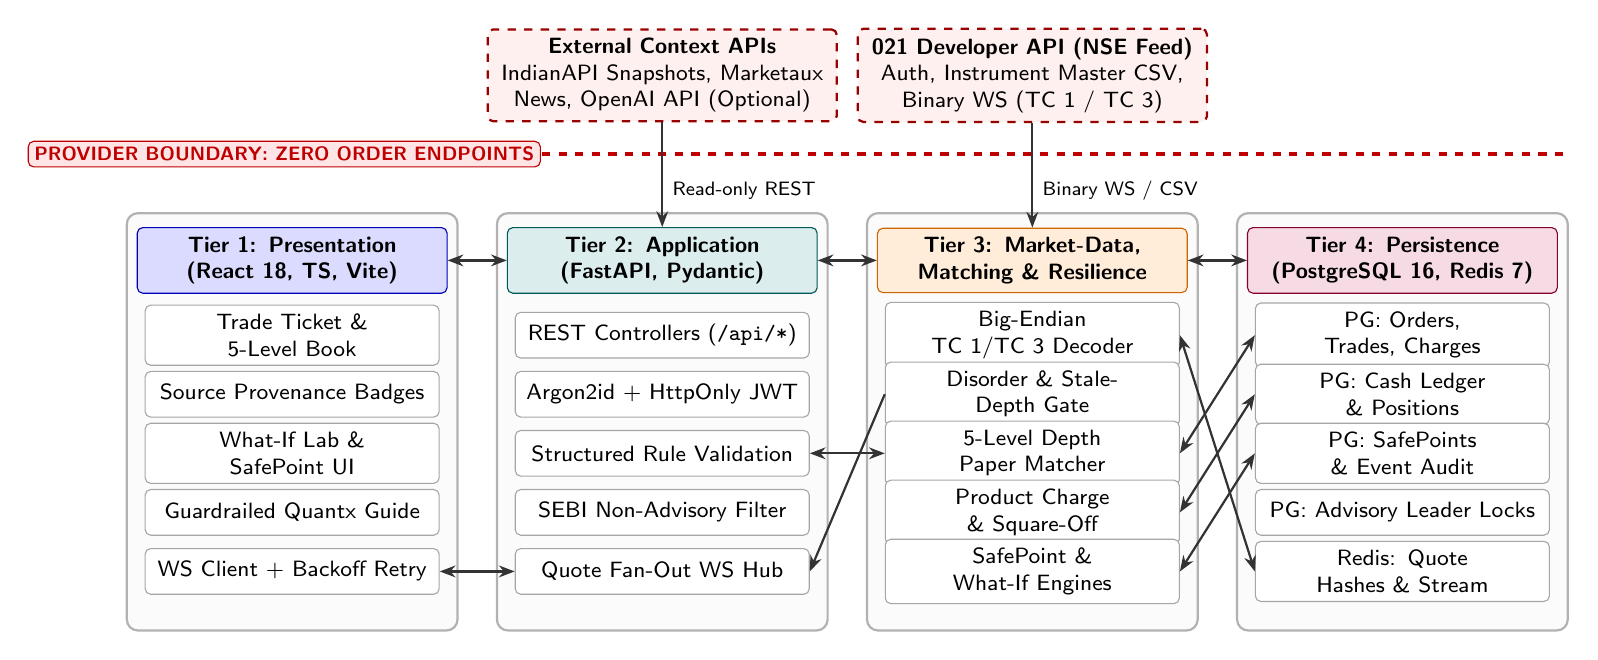
\begin{tikzpicture}[
  font=\footnotesize\sffamily,
  tierbox/.style={draw=gray!60, rounded corners=4pt, line width=0.8pt, fill=gray!3},
  hdr1/.style={draw=blue!70!black, fill=blue!14, rounded corners=2pt, minimum width=3.9cm, minimum height=0.75cm, text width=3.7cm, align=center, font=\footnotesize\sffamily\bfseries},
  hdr2/.style={draw=teal!70!black, fill=teal!14, rounded corners=2pt, minimum width=3.9cm, minimum height=0.75cm, text width=3.7cm, align=center, font=\footnotesize\sffamily\bfseries},
  hdr3/.style={draw=orange!80!black, fill=orange!15, rounded corners=2pt, minimum width=3.9cm, minimum height=0.75cm, text width=3.7cm, align=center, font=\footnotesize\sffamily\bfseries},
  hdr4/.style={draw=purple!70!black, fill=purple!14, rounded corners=2pt, minimum width=3.9cm, minimum height=0.75cm, text width=3.7cm, align=center, font=\footnotesize\sffamily\bfseries},
  itm/.style={draw=gray!70, fill=white, rounded corners=2pt, minimum width=3.7cm, minimum height=0.58cm, text width=3.5cm, align=center},
  ext/.style={draw=red!60!black, dashed, line width=0.8pt, fill=red!6, rounded corners=2pt, minimum width=4.4cm, minimum height=0.75cm, text width=4.2cm, align=center},
  arr/.style={-{Stealth[length=2.0mm]}, line width=0.8pt, draw=black!80},
  biarr/.style={{Stealth[length=2.0mm]}-{Stealth[length=2.0mm]}, line width=0.8pt, draw=black!80}
]

% Tier background frames
\draw[tierbox] (-2.1,-4.7) rectangle (2.1,0.6);
\draw[tierbox] (2.6,-4.7) rectangle (6.8,0.6);
\draw[tierbox] (7.3,-4.7) rectangle (11.5,0.6);
\draw[tierbox] (12.0,-4.7) rectangle (16.2,0.6);

% External Providers above boundary
\node[ext] (extA) at (4.7, 2.35) {\textbf{External Context APIs}\\IndianAPI Snapshots, Marketaux News, OpenAI API (Optional)};
\node[ext] (extB) at (9.4, 2.35) {\textbf{021 Developer API (NSE Feed)}\\Auth, Instrument Master CSV, Binary WS (TC~1 / TC~3)};

% Provider Boundary Line
\draw[red!75!black, dashed, line width=1.2pt] (-2.1, 1.35) -- (16.2, 1.35);
\node[fill=red!10, draw=red!75!black, rounded corners=2pt, inner sep=2.2pt, font=\scriptsize\sffamily\bfseries, text=red!75!black] at (-0.1, 1.35) {PROVIDER BOUNDARY: ZERO ORDER ENDPOINTS};

% Tier Headers
\node[hdr1] (h1) at (0, 0) {Tier 1: Presentation\\(React 18, TS, Vite)};
\node[hdr2] (h2) at (4.7, 0) {Tier 2: Application\\(FastAPI, Pydantic)};
\node[hdr3] (h3) at (9.4, 0) {Tier 3: Market-Data, Matching \& Resilience};
\node[hdr4] (h4) at (14.1, 0) {Tier 4: Persistence\\(PostgreSQL 16, Redis 7)};

% Tier 1 Items
\node[itm] (t1_1) at (0, -0.95) {Trade Ticket \& 5-Level Book};
\node[itm] (t1_2) at (0, -1.70) {Source Provenance Badges};
\node[itm] (t1_3) at (0, -2.45) {What-If Lab \& SafePoint UI};
\node[itm] (t1_4) at (0, -3.20) {Guardrailed Quantx Guide};
\node[itm] (t1_5) at (0, -3.95) {WS Client + Backoff Retry};

% Tier 2 Items
\node[itm] (t2_1) at (4.7, -0.95) {REST Controllers (\texttt{/api/*})};
\node[itm] (t2_2) at (4.7, -1.70) {Argon2id + HttpOnly JWT};
\node[itm] (t2_3) at (4.7, -2.45) {Structured Rule Validation};
\node[itm] (t2_4) at (4.7, -3.20) {SEBI Non-Advisory Filter};
\node[itm] (t2_5) at (4.7, -3.95) {Quote Fan-Out WS Hub};

% Tier 3 Items
\node[itm] (t3_1) at (9.4, -0.95) {Big-Endian TC~1/TC~3 Decoder};
\node[itm] (t3_2) at (9.4, -1.70) {Disorder \& Stale-Depth Gate};
\node[itm] (t3_3) at (9.4, -2.45) {5-Level Depth Paper Matcher};
\node[itm] (t3_4) at (9.4, -3.20) {Product Charge \& Square-Off};
\node[itm] (t3_5) at (9.4, -3.95) {SafePoint \& What-If Engines};

% Tier 4 Items
\node[itm] (t4_1) at (14.1, -0.95) {PG: Orders, Trades, Charges};
\node[itm] (t4_2) at (14.1, -1.70) {PG: Cash Ledger \& Positions};
\node[itm] (t4_3) at (14.1, -2.45) {PG: SafePoints \& Event Audit};
\node[itm] (t4_4) at (14.1, -3.20) {PG: Advisory Leader Locks};
\node[itm] (t4_5) at (14.1, -3.95) {Redis: Quote Hashes \& Stream};

% Arrows between external and tiers
\draw[arr] (extA.south) -- node[right, pos=0.65, font=\scriptsize\sffamily]{Read-only REST} (h2.north);
\draw[arr] (extB.south) -- node[right, pos=0.65, font=\scriptsize\sffamily]{Binary WS / CSV} (h3.north);

% Horizontal inter-tier arrows
\draw[biarr] (h1.east) -- (h2.west);
\draw[biarr] (h2.east) -- (h3.west);
\draw[biarr] (h3.east) -- (h4.west);

\draw[biarr] (t1_5.east) -- (t2_5.west);
\draw[arr] (t3_2.west) -- (t2_5.east);
\draw[biarr] (t2_3.east) -- (t3_3.west);
\draw[biarr] (t3_3.east) -- (t4_1.west);
\draw[biarr] (t3_4.east) -- (t4_2.west);
\draw[biarr] (t3_5.east) -- (t4_3.west);
\draw[biarr] (t3_1.east) -- (t4_5.west);

\end{tikzpicture}}
\caption{Quantx four-tier system architecture illustrating the strict read-only provider boundary above the application, the presentation and FastAPI control tiers, the in-process market-data decoding, depth-matching, SafePoint recovery, and What-If resilience tier, and the authoritative PostgreSQL/Redis persistence tier.}
\label{fig:arch}
\end{figure*}

\subsection{Separation of Responsibilities}
The architecture enforces an invariant separation between the \emph{market-data plane} and the \emph{accounting and resilience plane}. The market-data plane (\texttt{MarketDataService}, \texttt{ProviderClient}) may authenticate to an external provider, synchronize the NSE instrument catalog, and ingest binary quote and depth frames; it has no access to order-placement endpoints, holds no user account state, and never writes to the financial ledger. Conversely, the accounting and resilience plane (\texttt{PaperTradingEngine}, \texttt{RecoveryEngine}, \texttt{ScenarioEngine}) alone creates or mutates orders, trades, statutory charge records, cash-ledger entries, positions, and SafePoint snapshots. It never treats a depth-less REST snapshot (\texttt{indianapi}) as executable market depth, never coerces a missing quote to a zero price, and tags every quote with an explicit provenance label (\texttt{021\_live}, \texttt{indianapi}, or \texttt{demo}) so the user interface always reflects data origin.

\section{Boundary-Enforced Market-Data Plane}

The market-data plane transforms upstream frames—which arrive in big-endian binary format, express prices in integer paise, and are subject to network duplication, reordering, and disconnections—into normalized, event-time-ordered, rupee-denominated quotes suitable for deterministic consumption by the matching engine. Fig.~\ref{fig:pipe} depicts the end-to-end ingestion, filtering, caching, and fan-out pipeline.

\begin{figure}[!t]
\centering
\resizebox{\columnwidth}{!}{%
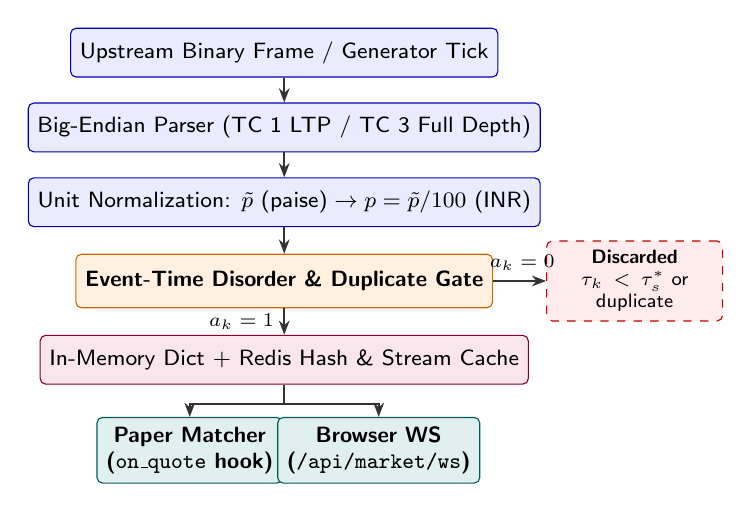
\begin{tikzpicture}[
  font=\footnotesize\sffamily,
  stepbox/.style={draw=blue!70!black, fill=blue!8, rounded corners=2pt, minimum width=4.5cm, minimum height=0.62cm, align=center},
  guardbox/.style={draw=orange!80!black, fill=orange!12, rounded corners=2pt, minimum width=4.5cm, minimum height=0.68cm, align=center, font=\footnotesize\sffamily\bfseries},
  cachebox/.style={draw=purple!70!black, fill=purple!10, rounded corners=2pt, minimum width=4.5cm, minimum height=0.62cm, align=center},
  sinkbox/.style={draw=teal!70!black, fill=teal!12, rounded corners=2pt, minimum width=2.15cm, minimum height=0.65cm, align=center, font=\footnotesize\sffamily\bfseries},
  dropbox/.style={draw=red!75!black, dashed, fill=red!8, rounded corners=2pt, minimum width=2.2cm, minimum height=0.85cm, text width=2.0cm, align=center, font=\scriptsize\sffamily},
  arr/.style={-{Stealth[length=1.8mm]}, line width=0.8pt, draw=black!80}
]
\node[stepbox] (s1) at (0, 0) {Upstream Binary Frame / Generator Tick};
\node[stepbox] (s2) at (0, -0.95) {Big-Endian Parser (TC~1 LTP / TC~3 Full Depth)};
\node[stepbox] (s3) at (0, -1.90) {Unit Normalization: $\tilde{p}\text{ (paise)} \rightarrow p = \tilde{p}/100\text{ (INR)}$};
\node[guardbox] (s4) at (0, -2.90) {Event-Time Disorder \& Duplicate Gate};
\node[cachebox] (s5) at (0, -3.90) {In-Memory Dict + Redis Hash \& Stream Cache};
\node[sinkbox] (k1) at (-1.20, -5.05) {Paper Matcher\\(\texttt{on\_quote} hook)};
\node[sinkbox] (k2) at (1.20, -5.05) {Browser WS\\(\texttt{/api/market/ws})};
\node[dropbox] (dr) at (4.45, -2.90) {\textbf{Discarded}\\$\tau_k < \tau^*_s$ or\\duplicate};

\draw[arr] (s1) -- (s2);
\draw[arr] (s2) -- (s3);
\draw[arr] (s3) -- (s4);
\draw[arr] (s4) -- node[left, font=\scriptsize\sffamily]{$a_k = 1$} (s5);
\draw[arr] (s4.east) -- node[above, pos=0.55, font=\scriptsize\sffamily]{$a_k=0$} (dr.west);
\draw[arr] (s5.south) -- ++(0,-0.25) -| (k1.north);
\draw[arr] (s5.south) -- ++(0,-0.25) -| (k2.north);
\end{tikzpicture}}
\caption{Boundary-enforced market-data pipeline from upstream binary frame to the local paper matcher and browser WebSocket hub, highlighting paise-to-rupee normalization, event-time disorder and duplicate filtering, and dual memory/Redis caching.}
\label{fig:pipe}
\end{figure}

\subsection{Provider Boundary and Source Provenance}
The backend authenticates to the upstream market-data provider (\texttt{021} Developer API) using server-held credentials to obtain a session token, synchronize the NSE cash equity instrument master CSV, and request a short-lived ephemeral key that opens the upstream WebSocket. Provider order-submission and order-update endpoints are excluded from the codebase. Every quote dictionary carries an explicit \texttt{data\_source} field:
\begin{enumerate}
  \item \texttt{021\_live}: Full five-level depth or last-traded-price packets streamed over the authenticated provider WebSocket.
  \item \texttt{indianapi}: Periodic REST price snapshots containing last price, high, low, and volume but zero order-book depth. The paper engine ignores these snapshots in \texttt{remember\_quote} and explicitly blocks \texttt{MARKET} orders against snapshot-only quotes (HTTP~409).
  \item \texttt{demo}: Deterministic-structure synthetic five-level depth generated every \thinunit{1.4}{s} per subscribed symbol when development mode is active, with per-level spread $\max\{0.025\%\text{ of last price},\,\thinunit{0.01}{INR}\}$, displayed quantities drawn uniformly from $[100,\,2{,}200]$ shares, and a bounded random-walk step within $\pm 0.09\%$. Fresh \texttt{021\_live} quotes automatically preempt \texttt{demo} ticks for the same symbol, and \texttt{demo\_market\_data\_enabled} is rejected by configuration validation when \texttt{app\_env="production"}.
\end{enumerate}

\subsection{Binary Frame Decoding and Unit Normalization}
The binary parser (\texttt{decode\_provider\_frame}) decodes big-endian packets for Transaction Code~1 (TC~1, last-traded-price header of 31~bytes) and Transaction Code~3 (TC~3, full cash/derivative packet of 171~bytes or index packet of 47~bytes); heartbeat frames (TC~10) are discarded. In full subscription mode (\texttt{subscribe\_full}), TC~3 packets for NSE cash equities carry ten 12-byte depth records—five bid levels followed by five ask levels—each containing unsigned 32-bit quantity, unsigned 32-bit price in paise, and unsigned 16-bit order count. Because provider packets and the NSE instrument master express all monetary values in integer paise whereas Quantx stores and displays rupee decimals, every price field is normalized at the ingestion boundary:
\begin{equation}
p = \frac{\tilde{p}}{100},
\label{eq:paise}
\end{equation}
where $\tilde{p}\in\mathbb{N}_0$ is the raw provider price or circuit bound (paise) and $p\in\mathbb{R}_{\ge 0}$ is the normalized rupee price (INR) quantized to $\thinunit{0.01}{INR}$. Share quantities and order counts remain unitless non-negative integers.

\subsection{Event-Time Disorder and Stale-Depth Guards}
Each decoded TC~3 packet carries an unsigned 32-bit exchange timestamp in seconds relative to the NSE epoch offset ($\Delta_{\mathrm{epoch}} = 315{,}513{,}000\,\text{s}$), which is converted to a UTC timestamp $\tau_k$; packets lacking an exchange timestamp (such as TC~1 frames) are stamped with the server receipt time upon arrival. For any instrument symbol $s$, let $\tau_k$ denote the exchange timestamp of arriving packet $k$ and $\tau^{*}_s$ denote the exchange timestamp of the currently cached quote. To prevent network reordering from regressing book state \cite{akidau2015,lamport1978}, the ingestion filter evaluates the acceptance indicator $a_k$:
\begin{equation}
a_k =
\begin{cases}
0, & \text{source}=\texttt{021\_live},\ \tau_k,\tau^{*}_s\text{ defined},\ \tau_k < \tau^{*}_s,\\
1, & \text{otherwise,}
\end{cases}
\label{eq:order}
\end{equation}
where $a_k\in\{0,1\}$ is the unitless acceptance decision and $\tau_k, \tau^{*}_s$ are UTC exchange timestamps (s). Packets with equal timestamps ($\tau_k = \tau^{*}_s$) but updated book state are admitted so sub-second depth revisions are preserved. Independently of timestamp comparison, the service computes a structural quote signature comprising \texttt{(data\_source, price, volume, bids, asks)} across all five bid and ask levels; any arriving \texttt{021\_live} or \texttt{demo} packet whose signature is identical to the cached signature for symbol $s$ is suppressed as a duplicate before touching Redis or the paper matcher.

At order-submission and matching time, the accounting plane enforces a staleness gate:
\begin{equation}
A_s(t) = t - \tau_s \le \theta,
\label{eq:stale}
\end{equation}
where $A_s(t)$ is the quote age at evaluation time $t$ (s), $\tau_s$ is the stored quote's effective timestamp (exchange timestamp when present, otherwise receipt timestamp, in UTC~s), $t$ is the backend host's UTC wall-clock time (s), and $\theta$ is the configured staleness threshold \texttt{market\_quote\_max\_age\_seconds} (default $\thinunit{120}{s}$). A missing or unparseable timestamp fails Equation~\eqref{eq:stale} unconditionally. Any user-submitted \texttt{MARKET} order for symbol $s$ when no quote is cached or when $A_s(t) > \theta$ is rejected immediately with HTTP~409, preventing market fills against frozen books. \texttt{LIMIT}, \texttt{SL}, and \texttt{SL-M} orders are admitted into the order book during stale intervals, but immediate matching is deferred until a fresh quote satisfying Equation~\eqref{eq:stale} arrives.

\subsection{Subscription Lifecycle and Multi-Worker Coordination}
A single upstream WebSocket connection to the provider is shared across all connected browsers, enforcing the provider's cap of 100 concurrent instrument subscriptions. A background retention loop (\texttt{\_subscription\_loop}) automatically retains upstream subscriptions for any symbol referenced by an open paper order or non-zero position even when all browser tabs disconnect. To support multi-worker deployments safely without duplicate upstream connections or duplicate intraday square-offs, Quantx acquires PostgreSQL session-level advisory locks (\texttt{pg\_try\_advisory\_lock} with keys \texttt{410021} for the market-data leader and \texttt{410022} for the operations worker). Accepted quotes are pushed to an in-process bounded queue ($10{,}000$ entries) consumed by a dedicated worker that invokes \texttt{paper\_engine.on\_quote} inside a worker thread and broadcasts JSON quote frames to subscribed browser WebSockets.

\section{Local Paper Matching, Statutory Charges, SafePoint Recovery, and Scenario Engines}

The accounting and resilience plane converts validated user intents into auditable ledger state transitions and provides non-destructive risk and recovery tools. Below we formalize each mechanism in execution order.

\subsection{Order Admission and Conservative Cash Reservation}
When \texttt{create\_order} receives a request, it executes a deterministic eight-step admission gate:
\begin{enumerate}
  \item \emph{Idempotency check:} Queries \texttt{orders.idempotency\_key}. If a matching row exists for the same account, the existing order is returned idempotently; if owned by a different account, HTTP~409 is raised \cite{helland2012}.
  \item \emph{Tradability check:} Verifies that the target \texttt{Instrument} exists, has \texttt{is\_tradable=True}, and holds a valid \texttt{provider\_token} (unless \texttt{demo\_market\_data\_enabled} is active).
  \item \emph{Tick normalization:} Converts the instrument's \texttt{tick\_size\_paise} to rupee tick $\Delta p = \max(\text{tick\_size\_paise}, 1)/100$ (INR) and rounds any supplied \texttt{limit\_price} or \texttt{trigger\_price} to the nearest valid tick via $\mathrm{round}(p/\Delta p)\cdot \Delta p$.
  \item \emph{Quantity, board-lot, and freeze validation:} Verifies that quantity $q_o \in \mathbb{N}$ satisfies $1 \le q_o \le q_{\mathrm{freeze}}$ and $q_o \bmod q_{\mathrm{lot}} = 0$, where $q_{\mathrm{lot}} = \max(\text{board\_lot\_quantity}, \text{lot\_size}, 1)$ and $q_{\mathrm{freeze}}$ is the instrument's NSE freeze quantity.
  \item \emph{Circuit-band validation:} For orders carrying a limit or trigger price, verifies $p_{\mathrm{lower}} \le p \le p_{\mathrm{upper}}$, where $p_{\mathrm{lower}}$ and $p_{\mathrm{upper}}$ are the instrument's lower and upper circuit limits in INR.
  \item \emph{Feed provenance and staleness gate:} Rejects \texttt{MARKET} orders if the quote source is \texttt{indianapi}, if no quote exists, or if Equation~\eqref{eq:stale} is violated (unless \texttt{allow\_stale\_market=True} is set by the internal 15:20~IST square-off worker).
  \item \emph{Stop-trigger directional consistency:} Against reference price $p_{\mathrm{ref}}$ (last traded price), verifies that a \texttt{BUY} stop has $p_{\mathrm{trig}} > p_{\mathrm{ref}}$ (and $p_{\mathrm{lim}} \ge p_{\mathrm{trig}}$ for \texttt{SL}), whereas a \texttt{SELL} stop has $p_{\mathrm{trig}} < p_{\mathrm{ref}}$ (and $p_{\mathrm{lim}} \le p_{\mathrm{trig}}$ for \texttt{SL}).
  \item \emph{Buying-power and holdings check:} For a \texttt{BUY} order, the engine computes a conservative cash reservation $R_o$:
\end{enumerate}
\begin{equation}
\begin{aligned}
R_o &= q_o\,p^{\mathrm{est}}_o\,(1+\rho)+\beta_o,\\
\rho &= \Bigl(\max\{t_{\mathrm{CNC}}+u_{\mathrm{CNC}},\,t_{\mathrm{MIS,S}}+u_{\mathrm{MIS}}\}\\
&\qquad +\epsilon_{\mathrm{X}}+\epsilon_{\mathrm{S}}+\phi\Bigr)(1+g),
\end{aligned}
\label{eq:reserve}
\end{equation}
where $R_o$ is the reserved cash amount for order $o$ (INR); $q_o\in\mathbb{N}$ is the order quantity (shares); $p^{\mathrm{est}}_o$ is the reservation reference price (INR), taken as the rounded \texttt{limit\_price} if present, else the highest visible ask price $\max_i \pi^{\mathrm{ask}}_i$, else the quote's last price; $\rho$ is the conservative upper-bound statutory charge ratio (unitless); $t_{\mathrm{CNC}}$ and $u_{\mathrm{CNC}}$ are the delivery STT and stamp-duty ratios; $t_{\mathrm{MIS,S}}$ and $u_{\mathrm{MIS}}$ are the intraday sell STT and buy stamp-duty ratios; $\epsilon_{\mathrm{X}}$, $\epsilon_{\mathrm{S}}$, $\phi$, and $g$ are the exchange, SEBI, account regulatory, and GST ratios defined in Equation~\eqref{eq:charge}; and $\beta_o$ is the per-order brokerage estimate (INR). A \texttt{BUY} order is admitted only if available cash satisfies $M_{\mathrm{cash}} - M_{\mathrm{res}} \ge R_o$. For a delivery (\texttt{CNC}) \texttt{SELL} order, the engine verifies that settled holdings minus open \texttt{CNC} sell orders cover $q_o$. Any admission failure raises HTTP~409 or~422 without persisting an order row.

\subsection{Five-Level Depth-Walking Matching}
When an admitted order is evaluated against a fresh quote, let the opposite side of the five-level book consist of levels $i\in\{1,\dots,5\}$ ordered best-price first (ascending ask prices $\pi_1 \le \dots \le \pi_5$ for a \texttt{BUY}; descending bid prices $\pi_1 \ge \dots \ge \pi_5$ for a \texttt{SELL}), with displayed share quantities $Q_i \in \mathbb{N}_0$ after any account-level stress transformation (Equation~\eqref{eq:stress}). For a \texttt{LIMIT} order (or a triggered \texttt{SL} order) with limit price $p_{\mathrm{lim}}$, the marketable level set is $E = \{i : \pi_i \le p_{\mathrm{lim}}\}$ for a \texttt{BUY} and $E = \{i : \pi_i \ge p_{\mathrm{lim}}\}$ for a \texttt{SELL}; for a \texttt{MARKET} order (or triggered \texttt{SL-M}), $E = \{1,\dots,5\}$. The matcher walks $i \in E$ sequentially and allocates fill quantity $x_i$:
\begin{equation}
x_i = \min\!\Bigl\{Q_i,\ \max\!\Bigl(0,\ q_{\mathrm{rem}}-\sum_{j\in E,\,j<i}x_j\Bigr)\Bigr\},\qquad i\in E,
\label{eq:alloc}
\end{equation}
where $x_i \in \mathbb{N}_0$ is the quantity filled at level $i$ (shares) and $q_{\mathrm{rem}} = q_o - q_{\mathrm{filled}}$ is the order's remaining unfilled quantity entering the pass (shares). The total pass fill quantity $f$ and volume-weighted average execution price $\bar{p}$ are:
\begin{align}
f &= \sum_{i\in E}x_i, \label{eq:filled}\\
\bar{p} &= \frac{1}{f}\sum_{i\in E}x_i\,\pi_i,\qquad f>0, \label{eq:vwap}
\end{align}
where $f\in\mathbb{N}_0$ is measured in shares and $\bar{p}$ in INR/share (quantized half-up to $\thinunit{0.01}{INR}$). Each level with $x_i > 0$ generates an individual \texttt{Trade} row with sequence index, execution price $\pi_i$, and level quantity $x_i$. If an order has validity \texttt{IOC}, any residual quantity $q_{\mathrm{rem}} - f > 0$ after walking $E$ is immediately cancelled and its remaining cash reservation is released; for \texttt{DAY} orders, the residual remains \texttt{OPEN} or \texttt{PARTIALLY\_FILLED} for subsequent quote ticks.

\subsection{Product-Aware Per-Fill Statutory Charges and Ledger Commit}
For each level fill $(x_i, \pi_i)$ with gross trade value $V = x_i\,\pi_i$ (INR), the fee routine (\texttt{\_calculate\_fees}) computes a six-component Indian statutory charge breakdown:
\begin{equation}
\begin{aligned}
C &= b\,\beta + \bigl(\epsilon_{\mathrm{X}} + \epsilon_{\mathrm{S}} + \phi + t_{k,d} + u_{k,d}\bigr)V\\
&\quad + g\Bigl(b\,\beta + (\epsilon_{\mathrm{X}} + \epsilon_{\mathrm{S}} + \phi)V\Bigr),\qquad V = x_i\,\pi_i,
\end{aligned}
\label{eq:charge}
\end{equation}
where $C$ is the total statutory and brokerage charge for the fill (INR); $V$ is the fill turnover (INR); $b\in\{0,1\}$ equals $1$ on the first fill of an order ($\text{filled\_quantity}=0$) and $0$ on subsequent partial fills of the same order; $\beta$ is the per-order brokerage (INR), equal to the account's custom \texttt{commission\_per\_order} if configured, otherwise $\thinunit{0.00}{INR}$ for \texttt{CNC} and $\min\{\thinunit{20.00}{INR},\,0.0003\,V\}$ for \texttt{MIS}; $\epsilon_{\mathrm{X}} = 0.0000325$ ($0.00325\%$) is the NSE exchange transaction charge ratio; $\epsilon_{\mathrm{S}} = 0.000001$ ($0.0001\%$) is the SEBI turnover fee ratio; $\phi = \text{regulatory\_fee\_percent}/100$ is the account's additional regulatory fee ratio; $t_{k,d}$ is the STT ratio for product $k\in\{\mathrm{CNC},\mathrm{MIS}\}$ and side $d\in\{\mathrm{BUY},\mathrm{SELL}\}$ ($0.001$ on both sides for \texttt{CNC}; $0.00025$ on \texttt{SELL} only for \texttt{MIS}); $u_{k,d}$ is the stamp-duty ratio ($0.00015$ on \texttt{CNC BUY}; $0.00003$ on \texttt{MIS BUY}; $0$ on \texttt{SELL}); and $g = 0.18$ ($18\%$) is the GST rate applied to brokerage, exchange fees, and SEBI/regulatory fees. Each of the six components (\texttt{brokerage}, \texttt{stt}, \texttt{exchange\_fee}, \texttt{sebi\_fee}, \texttt{stamp\_duty}, \texttt{gst}) is individually quantized half-up to $\thinunit{0.01}{INR}$ before summing into $C$.

The account's cash balance $M_{\mathrm{cash}}$ changes by:
\begin{equation}
\Delta M = -\,d_{\pm}\,x_i\,\pi_i - C,
\label{eq:cash}
\end{equation}
where $\Delta M$ is the net cash change (INR) and $d_{\pm} = +1$ for a \texttt{BUY} and $-1$ for a \texttt{SELL}. The engine writes two immutable \texttt{CashLedger} rows per fill—a \texttt{TRADE\_DEBIT} or \texttt{TRADE\_CREDIT} row for $\mp x_i\pi_i$ (keyed by \texttt{trade-gross:<trade\_id>}) and a \texttt{CHARGE} row for $-C$ (keyed by \texttt{trade-charge:<trade\_id>})—and commits the \texttt{Order}, \texttt{Trade}, \texttt{TradeCharge}, \texttt{OrderEvent}, \texttt{Position}, and \texttt{CashLedger} mutations within a single PostgreSQL transaction \cite{gray1993}.

\subsection{Signed Positions and Charge-Capitalized Realized P\&L}
Statutory charges are capitalized into an effective per-share execution price $p_{\mathrm{eff}} = \pi_i + d_{\pm}\,C/x_i$ (INR/share). For an existing position with signed share quantity $Q \in \mathbb{Z}$ ($Q>0$ long, $Q<0$ short) and average cost basis $A \in \mathbb{R}_{\ge 0}$ (INR/share), a fill that opens or adds to the same direction updates the cost basis and signed quantity as:
\begin{equation}
A' = \frac{|Q|\,A + x_i\,p_{\mathrm{eff}}}{|Q'|},\qquad Q' = Q + d_{\pm}\,x_i,
\label{eq:avg}
\end{equation}
where $A'$ is the new average cost basis (INR/share) and $Q'$ is the updated signed position quantity (shares). A fill opposing the current position direction closes $c = \min(|Q|, x_i)$ shares and increments cumulative realized profit and loss by:
\begin{equation}
P_{\mathrm{real}} = \mathrm{sgn}(Q)\,(p_{\mathrm{eff}}-A)\,c,
\label{eq:pnl}
\end{equation}
where $P_{\mathrm{real}}$ is the realized profit and loss (INR) and $\mathrm{sgn}(Q) \in \{+1,-1\}$ is the sign of the prior position. If the fill flattens the position ($Q'=0$), $A'$ resets to $0$; if the fill flips the sign of $Q$ ($x_i > |Q|$), the residual $x_i - |Q|$ opens a new position in direction $d_{\pm}$ at average basis $A' = p_{\mathrm{eff}}$.

\subsection{Market Stress Mode, Multi-Modal What-If Lab, and Transactional SafePoint Recovery}
\textbf{1) Account-Level Market Stress Mode:} When a learner enables Stress Mode on their account, simulated execution depth is degraded exclusively for that account prior to Equation~\eqref{eq:alloc}:
\begin{equation}
\begin{aligned}
\pi'_i &= \pi_i + s\,p_{\mathrm{last}} \ \text{(asks)},\\
\pi'_i &= \max\{0.01,\ \pi_i - s\,p_{\mathrm{last}}\} \ \text{(bids)},\\
Q'_i &= \lfloor \lambda\,Q_i \rfloor,
\end{aligned}
\label{eq:stress}
\end{equation}
where $\pi'_i$ (INR) and $Q'_i$ (shares) are the stressed level price and quantity, $p_{\mathrm{last}}$ is the quote's last price (INR), $s$ is \texttt{paper\_stress\_spread\_percent} (default $0.005$, shifting each side by $0.5\%$ of $p_{\mathrm{last}}$), and $\lambda$ is \texttt{paper\_stress\_liquidity\_factor} (default $0.5$, halving displayed depth).

\textbf{2) Multi-Modal What-If Scenario Laboratory:} Quantx provides two complementary, strictly read-only scenario engines that project hypothetical shocks without mutating ledger state. First, the portfolio holding shock engine (\texttt{/api/scenarios}) evaluates symbol-specific percentage shocks $\delta_j$ (\%) across each held position $j$ with quantity $q_j$ (shares) and current price $p_j$ (INR):
\begin{equation}
\begin{aligned}
V^{\mathrm{proj}}_j &= q_j\,\max\Bigl\{0,\ p_j\Bigl(1+\frac{\delta_j}{100}\Bigr)\Bigr\},\\
\Pi_j &= V^{\mathrm{proj}}_j - q_j\,p_j,
\end{aligned}
\label{eq:whatif}
\end{equation}
where $V^{\mathrm{proj}}_j$ is the projected holding valuation (INR) and $\Pi_j$ is the projected holding P\&L delta (INR). Second, the multi-modal What-If laboratory (\texttt{ScenarioEngine}, \texttt{/api/what-if/*}) supports three interactive analytical modes: (i) \emph{Single-Stock Scenario Grid}, which evaluates a $3\times 3$ matrix of price moves $\Delta p \in \{-5\%, 0\%, +5\%\}$ and volatility shifts $\Delta \sigma \in \{-10\%, 0\%, +10\%\}$ around user-specified moves; (ii) \emph{Portfolio Stress Test}, which combines a global market shift $\delta_{\mathrm{mkt}}$ (\%), a sector shift $\delta_{\mathrm{sec}}$ (\%), and stock overrides; and (iii) \emph{Capital Allocation Concentration Analysis}, which computes portfolio Herfindahl--Hirschman concentration and top-holding weight $w_{\max} = \max_j (V_j / \sum_k V_k)$, flagging high concentration risk when $w_{\max} > 0.35$.

\textbf{3) Transactional SafePoint Recovery Shield:} To allow learners to experiment with aggressive order structures or stress scenarios and recover cleanly, \texttt{RecoveryEngine} (\texttt{/api/recovery/*}) implements atomic portfolio checkpointing and autonomous fault recovery. Creating a SafePoint $S_m$ captures a serialized JSON state vector:
\begin{equation}
S_m = \bigl(M^{(m)}_{\mathrm{cash}},\ M^{(m)}_{\mathrm{res}},\ \mathcal{P}^{(m)},\ \mathcal{O}^{(m)}_{\mathrm{open}}\bigr),
\label{eq:safepoint}
\end{equation}
where $M^{(m)}_{\mathrm{cash}}$ and $M^{(m)}_{\mathrm{res}}$ are the account's cash and reserved balances (INR) at capture time $t_m$, $\mathcal{P}^{(m)} = \{(i_r, k_r, Q_r, A_r, P_{\mathrm{real},r})\}_{r=1}^{R_m}$ is the set of active position tuples, and $\mathcal{O}^{(m)}_{\mathrm{open}}$ is the set of open orders. Before executing a rollback, the user can request a dry-run diff (\texttt{/api/recovery/diff}), which computes the exact cash restoration delta and per-symbol quantity adjustment:
\begin{equation}
\Delta M_{\mathrm{restore}} = M^{(m)}_{\mathrm{cash}} - M_{\mathrm{cash}}(t),\quad \Delta Q_{s} = Q^{(m)}_{s} - Q_{s}(t),
\label{eq:rollback}
\end{equation}
where $\Delta M_{\mathrm{restore}}$ (INR) is the cash balance adjustment and $\Delta Q_{s}$ (shares) is the position delta for symbol $s$. Executing rollback (\texttt{execute\_rollback}) runs inside a single database transaction: it cancels all currently \texttt{OPEN}, \texttt{PENDING}, or \texttt{PARTIALLY\_FILLED} orders, restores $M_{\mathrm{cash}} \leftarrow M^{(m)}_{\mathrm{cash}}$ and $M_{\mathrm{res}} \leftarrow \thinunit{0.00}{INR}$, replaces current positions with $\mathcal{P}^{(m)}$, and appends an auditable \texttt{RESET} entry to \texttt{cash\_ledger}. Furthermore, an autonomous recovery daemon (\texttt{simulate\_fault\_and\_recover}) detects three classes of simulated runtime faults—\texttt{DATA\_CORRUPTION} (non-numeric price injection), \texttt{OVERLOAD} (500-order burst congestion), and \texttt{CONCURRENCY} (conflicting state mutation)—and automatically executes a transactional rollback to the latest healthy SafePoint. Fig.~\ref{fig:resilience} illustrates the SafePoint Recovery Shield and Multi-Modal What-If pipeline.

\begin{figure}[!t]
\centering
\resizebox{\columnwidth}{!}{%
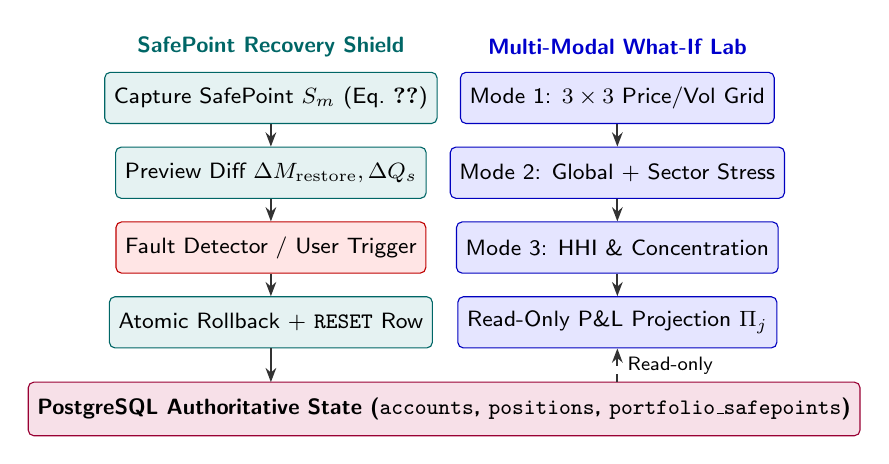
\begin{tikzpicture}[
  font=\footnotesize\sffamily,
  spbox/.style={draw=teal!80!black, fill=teal!10, rounded corners=2pt, minimum width=3.9cm, minimum height=0.65cm, align=center},
  fltbox/.style={draw=red!75!black, fill=red!10, rounded corners=2pt, minimum width=3.9cm, minimum height=0.65cm, align=center},
  wibox/.style={draw=blue!75!black, fill=blue!10, rounded corners=2pt, minimum width=3.9cm, minimum height=0.65cm, align=center},
  dbbox/.style={draw=purple!80!black, fill=purple!12, rounded corners=2pt, minimum width=8.3cm, minimum height=0.68cm, align=center, font=\footnotesize\sffamily\bfseries},
  arr/.style={-{Stealth[length=1.8mm]}, line width=0.8pt, draw=black!80}
]
% Left column: SafePoint Recovery Shield
\node[font=\footnotesize\sffamily\bfseries, text=teal!80!black] at (-2.2, 0.65) {SafePoint Recovery Shield};
\node[spbox] (sp1) at (-2.2, 0) {Capture SafePoint $S_m$ (Eq.~\ref{eq:safepoint})};
\node[spbox] (sp2) at (-2.2, -0.95) {Preview Diff $\Delta M_{\mathrm{restore}}, \Delta Q_s$};
\node[fltbox] (sp3) at (-2.2, -1.90) {Fault Detector / User Trigger};
\node[spbox] (sp4) at (-2.2, -2.85) {Atomic Rollback + \texttt{RESET} Row};

% Right column: Multi-Modal What-If Lab
\node[font=\footnotesize\sffamily\bfseries, text=blue!80!black] at (2.2, 0.65) {Multi-Modal What-If Lab};
\node[wibox] (wi1) at (2.2, 0) {Mode 1: $3\times 3$ Price/Vol Grid};
\node[wibox] (wi2) at (2.2, -0.95) {Mode 2: Global + Sector Stress};
\node[wibox] (wi3) at (2.2, -1.90) {Mode 3: HHI \& Concentration};
\node[wibox] (wi4) at (2.2, -2.85) {Read-Only P\&L Projection $\Pi_j$};

% Bottom shared DB bar
\node[dbbox] (db) at (0, -3.95) {PostgreSQL Authoritative State (\texttt{accounts}, \texttt{positions}, \texttt{portfolio\_safepoints})};

\draw[arr] (sp1) -- (sp2);
\draw[arr] (sp2) -- (sp3);
\draw[arr] (sp3) -- (sp4);
\draw[arr] (sp4.south) -- (-2.2, -3.61);

\draw[arr] (wi1) -- (wi2);
\draw[arr] (wi2) -- (wi3);
\draw[arr] (wi3) -- (wi4);
\draw[arr, dashed] (2.2, -3.61) -- node[right, font=\scriptsize\sffamily]{Read-only} (wi4.south);
\end{tikzpicture}}
\caption{Dual resilience architecture showing (left) the transactional SafePoint Recovery Shield that captures portfolio snapshots, computes pre-rollback diffs, and executes atomic state rollbacks, and (right) the strictly read-only Multi-Modal What-If Scenario Laboratory.}
\label{fig:resilience}
\end{figure}

\section{Runtime Configuration, Structured Validation, and Guardrailed Assistance}

Every paper order traverses a deterministic four-phase execution pipeline, illustrated in Fig.~\ref{fig:phases}. In \textbf{Phase~1 (Ingestion \& Normalization)}, the backend authenticates the HTTP/WebSocket session, decodes incoming TC~1/TC~3 binary frames, normalizes paise to INR, and parses the order payload. In \textbf{Phase~2 (Rule Gate \& Cash Reservation)}, the admission gate enforces idempotency, tradability, tick rounding, board-lot and freeze bounds, circuit bands, quote provenance and staleness ($\theta=\thinunit{120}{s}$), stop-trigger direction, and conservative cash reservation $R_o$; any violation aborts execution and returns a structured HTTP~409/422 error with zero state mutation. In \textbf{Phase~3 (Depth-Walking Matching \& Statutory Charges)}, the matcher walks up to five book levels, handles \texttt{IOC} remainders, and computes the six-component product-aware statutory charge vector. In \textbf{Phase~4 (Transactional Commit \& Real-Time Sync)}, the engine writes all order, trade, charge, event, position, and cash-ledger records inside a single PostgreSQL transaction and pushes updated state to the client workspace.

\begin{figure*}[!t]
\centering
\resizebox{\textwidth}{!}{%
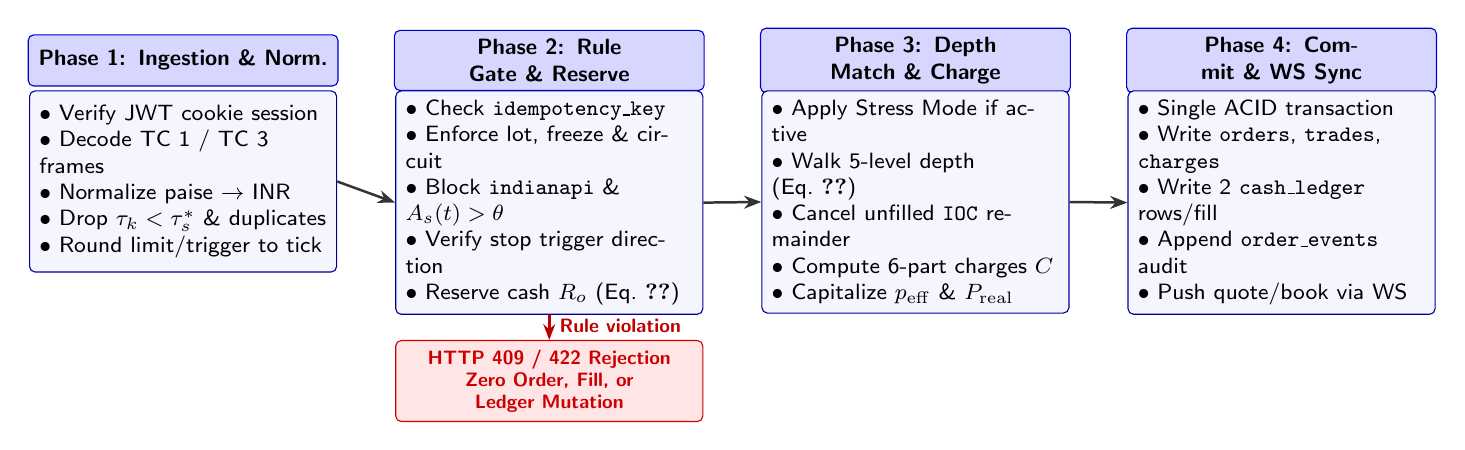
\begin{tikzpicture}[
  font=\footnotesize\sffamily,
  phhdr/.style={draw=blue!80!black, fill=blue!16, rounded corners=2pt, minimum width=3.9cm, minimum height=0.65cm, text width=3.7cm, align=center, font=\footnotesize\sffamily\bfseries},
  phbody/.style={draw=blue!60!black, fill=blue!4, rounded corners=2pt, minimum width=3.9cm, minimum height=2.30cm, text width=3.65cm, align=left},
  rejbox/.style={draw=red!80!black, fill=red!10, rounded corners=2pt, minimum width=3.9cm, minimum height=0.80cm, text width=3.65cm, align=center, font=\scriptsize\sffamily\bfseries, text=red!80!black},
  arr/.style={-{Stealth[length=2.2mm]}, line width=0.9pt, draw=black!80},
  rejarr/.style={-{Stealth[length=2.0mm]}, line width=0.9pt, draw=red!75!black}
]

% Phase 1
\node[phhdr] (h1) at (0, 0) {Phase 1: Ingestion \& Norm.};
\node[phbody, anchor=north] (b1) at (0, -0.38) {
  $\bullet$ Verify JWT cookie session\\
  $\bullet$ Decode TC~1 / TC~3 frames\\
  $\bullet$ Normalize paise $\rightarrow$ INR\\
  $\bullet$ Drop $\tau_k < \tau^*_s$ \& duplicates\\
  $\bullet$ Round limit/trigger to tick
};

% Phase 2
\node[phhdr] (h2) at (4.65, 0) {Phase 2: Rule Gate \& Reserve};
\node[phbody, anchor=north] (b2) at (4.65, -0.38) {
  $\bullet$ Check \texttt{idempotency\_key}\\
  $\bullet$ Enforce lot, freeze \& circuit\\
  $\bullet$ Block \texttt{indianapi} \& $A_s(t)>\theta$\\
  $\bullet$ Verify stop trigger direction\\
  $\bullet$ Reserve cash $R_o$ (Eq.~\ref{eq:reserve})
};

% Phase 3
\node[phhdr] (h3) at (9.30, 0) {Phase 3: Depth Match \& Charge};
\node[phbody, anchor=north] (b3) at (9.30, -0.38) {
  $\bullet$ Apply Stress Mode if active\\
  $\bullet$ Walk 5-level depth (Eq.~\ref{eq:alloc})\\
  $\bullet$ Cancel unfilled \texttt{IOC} remainder\\
  $\bullet$ Compute 6-part charges $C$\\
  $\bullet$ Capitalize $p_{\mathrm{eff}}$ \& $P_{\mathrm{real}}$
};

% Phase 4
\node[phhdr] (h4) at (13.95, 0) {Phase 4: Commit \& WS Sync};
\node[phbody, anchor=north] (b4) at (13.95, -0.38) {
  $\bullet$ Single ACID transaction\\
  $\bullet$ Write \texttt{orders}, \texttt{trades}, \texttt{charges}\\
  $\bullet$ Write 2 \texttt{cash\_ledger} rows/fill\\
  $\bullet$ Append \texttt{order\_events} audit\\
  $\bullet$ Push quote/book via WS
};

% Rejection sink below Phase 2
\node[rejbox, anchor=north] (rej) at (4.65, -3.55) {HTTP 409 / 422 Rejection\\Zero Order, Fill, or Ledger Mutation};

% Connections
\draw[arr] (b1.east) -- (b2.west);
\draw[arr] (b2.east) -- (b3.west);
\draw[arr] (b3.east) -- (b4.west);
\draw[rejarr] (b2.south) -- node[right, pos=0.45, font=\scriptsize\sffamily\bfseries, text=red!75!black]{Rule violation} (rej.north);

\end{tikzpicture}}
\caption{Four-phase Quantx order-execution workflow detailing session and frame ingestion, the eight-point admission and cash-reservation rule gate, five-level depth-walking matching with Indian statutory charge computation, and single-transaction PostgreSQL persistence with WebSocket synchronization.}
\label{fig:phases}
\end{figure*}

TABLE~\ref{tab:config} documents the runtime configuration parameters across all backend modules, and TABLE~\ref{tab:fields} specifies the validated order-submission contract. The complete API and database schemas are provided in Appendix~A.

\begin{table}[!t]
\caption{Module Configuration Parameters}
\label{tab:config}
\centering
\small
\renewcommand{\arraystretch}{1.12}
\begin{tabularx}{\columnwidth}{@{}>{\raggedright\arraybackslash}p{0.98in}X@{}}
\toprule
Module & Configured values in active codebase \\
\midrule
Market feed & Full mode (\texttt{subscribe\_full}); 5 bid / 5 ask levels; TC~1 (31\,B) and TC~3 (171\,B/47\,B) decoded; TC~10 ignored; max 100 concurrent instruments; advisory lock \texttt{410021} \\
Staleness guard & $\theta=$ \texttt{market\_quote\_max\_age\_seconds}, default \thinunit{120}{s} \\
Statutory charges$^{\dagger}$ & Exchange $\epsilon_{\mathrm{X}}=0.0000325$; SEBI $\epsilon_{\mathrm{S}}=0.000001$; GST $g=0.18$ on $(\beta+\epsilon_{\mathrm{X}}+\epsilon_{\mathrm{S}}+\phi)$; CNC: STT $0.001$ both sides, stamp $0.00015$ buy, brokerage $\thinunit{0}{INR}$; MIS: STT $0.00025$ sell, stamp $0.00003$ buy, brokerage $\min\{\thinunit{20}{INR}, 0.0003V\}$ on first fill; custom account commission/regulatory fee supported \\
Stress mode & Spread multiplier $s=0.005$ of $p_{\mathrm{last}}$; liquidity factor $\lambda=0.5$; per-account toggle \\
MIS square-off & Weekdays $\ge$ 15:20~IST, polled every \thinunit{10}{s}; idempotent key \texttt{auto-squareoff:<date>:<pos\_id>}; advisory lock \texttt{410022} \\
Capital & Allowed presets from INR 100,000 to 5,000,000; SafePoint JSON snapshots in \texttt{portfolio\_safepoints} \\
What-If Lab & Single-stock $3\times 3$ price/volatility grid; portfolio global/sector stress; concentration risk threshold $w_{\max} > 0.35$ \\
Quantx Guide & Dual-mode (\texttt{market\_guide} / \texttt{support}); regex + prompt guardrails blocking buy/sell investment advice; max 6 history turns \\
Auth \& recovery & Argon2id password hash; \texttt{HttpOnly}, \texttt{SameSite=Lax} JWT cookie; SHA-256 reset token (\thinunit{30}{min} TTL, 1 req/min throttle) \\
\bottomrule
\end{tabularx}

\vspace{2pt}
{\footnotesize $^{\dagger}$Statutory ratios in \texttt{PaperTradingEngine.\_calculate\_fees}; \texttt{PAPER\_*} environment settings parameterize the conservative reservation ratio $\rho$ in Equation~\eqref{eq:reserve}.}
\end{table}

\begin{table}[!t]
\caption{Validated Order Request Fields (\texttt{OrderCreateInput})}
\label{tab:fields}
\centering
\small
\renewcommand{\arraystretch}{1.12}
\begin{tabularx}{\columnwidth}{@{}>{\raggedright\arraybackslash}p{1.15in}X@{}}
\toprule
Field & Purpose and enforced validation constraint \\
\midrule
\texttt{instrument\_id} & Instrument primary key (UUID string); must reference an active, tradable NSE instrument \\
\texttt{side} & Order direction: \texttt{BUY} or \texttt{SELL} \\
\texttt{product} & \texttt{CNC} (cash delivery) or \texttt{MIS} (intraday square-off); governs STT, stamp duty, brokerage, and 15:20~IST auto-exit \\
\texttt{order\_type} & \texttt{MARKET}, \texttt{LIMIT}, \texttt{SL} (stop-limit), or \texttt{SL-M} (stop-market) \\
\texttt{quantity} & Integer in $[1,\,1{,}000{,}000]$ shares; exact multiple of board lot $q_{\mathrm{lot}}$; bounded by $q_o \le q_{\mathrm{freeze}}$ \\
\texttt{limit\_price} & Positive decimal (INR); required for \texttt{LIMIT}/\texttt{SL}, forbidden for \texttt{MARKET}/\texttt{SL-M}; tick-rounded; inside $[p_{\mathrm{lower}}, p_{\mathrm{upper}}]$ \\
\texttt{trigger\_price} & Positive decimal (INR); required for \texttt{SL}/\texttt{SL-M}, forbidden otherwise; tick-rounded; directional stop check vs.\ $p_{\mathrm{last}}$ \\
\texttt{validity} & \texttt{DAY} (default) or \texttt{IOC} (unfilled remainder cancelled immediately) \\
\texttt{idempotency\_key} & String of 8--64 characters; unique across \texttt{orders}; same-account repeat returns existing order, cross-account raises HTTP~409 \\
\bottomrule
\end{tabularx}
\end{table}

\subsection{Order Lifecycle, Idempotency, and Guardrailed Quantx Guide}
Fig.~\ref{fig:fsm} depicts the order-status state machine combined with the SafePoint rollback transition. Admitted orders enter \texttt{OPEN} (or reject at the HTTP gate without creating a database row), transition through \texttt{PARTIALLY\_FILLED} to \texttt{FILLED} as depth levels are consumed, or transition to \texttt{CANCELLED} via user cancellation, \texttt{IOC} remainder expiry, or a SafePoint rollback. Every state transition appends a structured JSON record to \texttt{order\_events} (\texttt{ACCEPTED}, \texttt{MODIFIED}, \texttt{TRIGGERED}, \texttt{PARTIAL\_FILL}, \texttt{FILL}, \texttt{FILLED}, \texttt{CANCELLED}).

\begin{figure}[!t]
\centering
\resizebox{\columnwidth}{!}{%
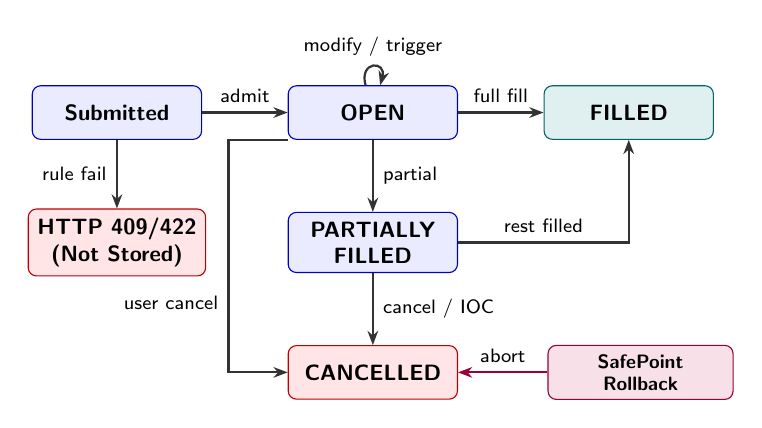
\begin{tikzpicture}[
  font=\footnotesize\sffamily,
  st/.style={draw=blue!75!black, fill=blue!8, rounded corners=3pt, minimum width=2.15cm, minimum height=0.68cm, align=center, font=\footnotesize\sffamily\bfseries},
  term/.style={draw=teal!80!black, fill=teal!12, rounded corners=3pt, minimum width=2.15cm, minimum height=0.68cm, align=center, font=\footnotesize\sffamily\bfseries},
  bad/.style={draw=red!75!black, fill=red!10, rounded corners=3pt, minimum width=2.15cm, minimum height=0.68cm, align=center, font=\footnotesize\sffamily\bfseries},
  sp/.style={draw=purple!80!black, fill=purple!12, rounded corners=3pt, minimum width=2.35cm, minimum height=0.68cm, align=center, font=\scriptsize\sffamily\bfseries},
  arr/.style={-{Stealth[length=1.8mm]}, line width=0.8pt, draw=black!80}
]
\node[st]   (sub) at (0, 0)      {Submitted};
\node[st]   (opn) at (3.25, 0)   {OPEN};
\node[term] (fil) at (6.50, 0)   {FILLED};
\node[bad]  (rej) at (0, -1.65)  {HTTP 409/422\\(Not Stored)};
\node[st]   (par) at (3.25, -1.65){PARTIALLY\\FILLED};
\node[bad]  (can) at (3.25, -3.30){CANCELLED};
\node[sp]   (rbk) at (6.65, -3.30){SafePoint\\Rollback};

\draw[arr] (sub) -- node[above, font=\scriptsize\sffamily]{admit} (opn);
\draw[arr] (opn) -- node[above, font=\scriptsize\sffamily]{full fill} (fil);
\draw[arr] (sub) -- node[left, font=\scriptsize\sffamily]{rule fail} (rej);
\draw[arr] (opn) -- node[right, font=\scriptsize\sffamily]{partial} (par);
\draw[arr] (par.east) -| node[above, pos=0.25, font=\scriptsize\sffamily]{rest filled} (fil.south);
\draw[arr] (par) -- node[right, font=\scriptsize\sffamily]{cancel / IOC} (can);
\draw[arr] (opn.south west) -- ++(-0.75,0) |- node[left, pos=0.35, font=\scriptsize\sffamily]{user cancel} (can.west);
\draw[arr] (opn) to[loop above, looseness=4.5] node[above, font=\scriptsize\sffamily]{modify / trigger} (opn);
\draw[arr, draw=purple!80!black] (rbk.west) -- node[above, font=\scriptsize\sffamily]{abort} (can.east);
\end{tikzpicture}}
\caption{Paper-order lifecycle and SafePoint rollback state machine showing admission, stop triggering, partial fills, IOC remainder cancellation, and atomic cancellation of open orders during SafePoint restoration.}
\label{fig:fsm}
\end{figure}

Finally, the workspace includes the \textbf{Quantx Guide} (\texttt{/api/support/chat}), a dual-mode educational and support assistant operating in \texttt{market\_guide} mode (explaining NSE market sessions, pre-open 09:00--09:15~IST, regular session 09:15--15:30~IST, circuit breakers, and product mechanics) and \texttt{support} mode (troubleshooting HTTP~409/422 order rejections, staleness blocks, and SafePoint recovery). To enforce SEBI regulatory boundaries between educational software and registered investment advisers, the service passes every user query through a deterministic advisory-intent filter (\texttt{\_asks\_for\_investment\_advice}) prior to knowledge retrieval or optional LLM formatting, refusing any request for buy/sell recommendations, target prices, or stock tips while offering to explain the underlying order-book or charge mechanics instead.

\section{Experimental Setup and System Evaluation}

We evaluated Quantx through a controlled, reproducible replay and microbenchmark suite executed directly against the containerized PostgreSQL~16.15 and Redis~7.4.11 stack. The primary goal is to audit whether the implemented pipeline satisfies Hypotheses H1--H3 and to quantify where a naive simulator baseline (B0) fails. TABLE~\ref{tab:env} documents the exact hardware and software environment used for all measurements.

\begin{table}[!t]
\caption{Evaluation Hardware and Software Environment}
\label{tab:env}
\centering
\small
\renewcommand{\arraystretch}{1.12}
\begin{tabularx}{\columnwidth}{@{}>{\raggedright\arraybackslash}p{1.05in}X@{}}
\toprule
Component & Verified specification \\
\midrule
Host CPU & Intel Core i5-8500T @ \thinunit{2.10}{GHz} (6 physical cores, 6 hardware threads) \\
Memory \& storage & \thinunit{8.0}{GB} DDR4 RAM (\thinunit{7.78}{GB} usable); \thinunit{512}{GB} WD PC SN5000S NVMe SSD \\
Operating system & Microsoft Windows 11 Pro (64-bit) with WSL2 Linux kernel backend \\
Container runtime & Docker Engine v29.9.2, Docker Compose v5.6.0 \\
Backend runtime & Python 3.12.15, FastAPI 0.156.8, Pydantic 2.14.1, SQLAlchemy 2.1.5, psycopg 3.3.6, uvicorn 0.54.0, argon2-cffi 25.1.0 \\
Frontend runtime & Node.js v24.19.0, React 18, TypeScript, Vite \\
Persistence stack & PostgreSQL 16.15 (\texttt{postgres:16-alpine}); Redis 7.4.11 (\texttt{redis:7-alpine}) \\
Recorded tick corpus & \texttt{recorded\_market\_ticks.jsonl} ($80{,}504$ lines, SHA-256 prefix \texttt{a9fd8616}); committed in initial snapshot \texttt{f89c99b} \\
\bottomrule
\end{tabularx}
\end{table}

\textbf{Provenance and Audit of Recorded Input.} The repository includes \texttt{backend/data/recorded\_market\_ticks.jsonl} ($80{,}504$ records across 100 NSE symbols, 804--806 records per symbol, spanning \thinunit{652.7}{s} with median inter-arrival \thinunit{6.3}{ms} and p99 \thinunit{26.3}{ms}) and \texttt{quote\_snapshots.json} (100 symbols). Forensic inspection of the codebase and git history (\texttt{f89c99b}) resolves the exact provenance of these files: \texttt{record\_market\_tick} is invoked exclusively by \texttt{MarketDataStore.update\_quote} when \texttt{source=="live"}, without passing an \texttt{exchange\_time} argument (so \texttt{exchange\_time} is \texttt{null} on all $80{,}504$ lines). Furthermore, receipt timestamps span \texttt{15:13:02Z}--\texttt{15:23:55Z} (\texttt{20:43:02}--\texttt{20:53:55~IST}), which lies outside NSE's regular trading session (\texttt{09:15}--\texttt{15:30~IST}), and the records contain no five-level bid/ask arrays, exhibit cyclic 100-symbol emission, include 151 zero-price ticks, and violate tick-size multiples on $30.9\%$ of positive prices. Consequently, we use \texttt{recorded\_market\_ticks.jsonl} strictly as an empirical inter-arrival and anomaly corpus, and construct deterministic five-level depth frames (\texttt{source="021\_live"}) across liquid NSE instruments (\texttt{RELIANCE}, \texttt{TCS}, \texttt{HDFCBANK}, \texttt{INFY}, \texttt{SBIN}) for controlled depth-walking and disorder evaluation.

\textbf{Controlled Scenario Profiles and Baseline B0.} Both Quantx and baseline B0 were initialized with identical virtual accounts ($\thinunit{5{,}000{,}000.00}{INR}$ starting capital) and subjected to $N=50$ valid scripted orders across three scenario profiles plus $N_{\mathrm{adv}}=50$ adversarial fault events:
\begin{enumerate}
  \item \emph{Typical Profile ($N_1=20$ orders):} Marketable \texttt{BUY} and \texttt{SELL} orders (10~\texttt{CNC}, 10~\texttt{MIS}; \texttt{MARKET} and \texttt{LIMIT}) with quantities $q_o \in [8,\,30]$ shares that fill completely within the best displayed level ($Q_1=100$ shares).
  \item \emph{Boundary Profile ($N_2=20$ orders):} Multi-level depth-walking orders ($q_o \in [60,\,250]$ shares across five levels of $Q_i=50$ shares each, generating $N_f=73$ total level fills across the $N=50$ valid orders), \texttt{IOC} orders with partial fills and immediate remainder cancellation, prices placed exactly on circuit and tick boundaries, and triggered \texttt{SL}/\texttt{SL-M} orders.
  \item \emph{Adversarial Profile ($N_3=10$ valid orders + $N_{\mathrm{adv}}=50$ injected faults):} Valid multi-level limit orders interleaved with 50 adversarial events: (i) $16$ out-of-order provider packets with $\tau_k < \tau^{*}_s$ and $8$ duplicate packets, (ii) $8$ \texttt{MARKET} orders submitted against stale quotes ($A_s(t) = \thinunit{300}{s} > \theta$), (iii) $7$ repeated submissions of an existing \texttt{idempotency\_key}, and (iv) $11$ rule-violating payloads (exceeding NSE freeze quantity, violating board-lot multiples, breaching upper/lower circuit bands, violating stop-trigger direction, or exceeding available buying power).
\end{enumerate}

Baseline \textbf{B0} implements the legacy naive simulator rules: it executes the full order quantity $q_o$ at the last traded price $p_{\mathrm{last}}$ in a single fill, charges $\thinunit{0.00}{INR}$ in statutory fees, overwrites cached quotes in arrival order regardless of $\tau_k$, applies no staleness check, ignores \texttt{idempotency\_key}, and omits circuit, lot, freeze, and buying-power gates. Expected reference fills, statutory charges, and cash balances ($M^{\mathrm{ref}}_n$) are computed by an independent reference oracle (\texttt{OracleEngine}) implementing Equations~\eqref{eq:paise}--\eqref{eq:cash} with identical half-up paisa quantization.

\subsection{Correctness and Resilience Audit}
TABLE~\ref{tab:correct} presents the empirical correctness audit comparing B0 and Quantx against the independent reference oracle across all $N=50$ valid orders ($N_f=73$ level fills in Quantx) and $N_{\mathrm{adv}}=50$ adversarial injections. At the end of the 50-order sequence, Quantx's authoritative PostgreSQL cash balance was $\thinunit{2{,}242{,}498.88}{INR}$, matching the independent oracle balance of $\thinunit{2{,}242{,}498.88}{INR}$ with an exact reconciliation difference of $\thinunit{0.00}{INR}$ ($\varepsilon_M = \thinunit{0.00}{INR} \le \thinunit{0.01}{INR}$, confirming \textbf{H1}). By contrast, B0 accumulated a mean cumulative ledger error of $\thinunit{19{,}684.41}{INR/order}$ (maximum $\thinunit{227{,}398.32}{INR}$) due to executing partially marketable limit orders in full at $p_{\mathrm{last}}$, ignoring five-level depth slippage ($\delta_p = \thinunit{1.60}{INR/share}$ mean, $\thinunit{9.51}{INR/share}$ max), and omitting statutory charges ($\thinunit{33.08}{INR/fill}$ mean, $\thinunit{116.01}{INR/fill}$ max). Under the Adversarial profile, Quantx recorded zero stale market-order executions, zero older-timestamp quote overwrites ($O=0$, confirming \textbf{H2}), zero duplicate effects from repeated idempotency keys, and zero accepted invalid orders (confirming \textbf{H3}).

\begin{table}[!t]
\caption{Correctness and Resilience Audit on Scripted Scenarios ($N=50$ Valid Orders, $N_f=73$ Fills, $N_{\mathrm{adv}}=50$ Faults)}
\label{tab:correct}
\centering
\small
\renewcommand{\arraystretch}{1.12}
\begin{tabularx}{\columnwidth}{@{}>{\raggedright\arraybackslash}X r r r@{}}
\toprule
Metric (unit) & B0 & Quantx & Diff. \\
\midrule
Ledger error, mean (INR/order) & 19,684.41 & 0.00 & $-$19,684.41 \\
Ledger error, max (INR/order) & 227,398.32 & 0.00 & $-$227,398.32 \\
Fill-price dev., mean (INR/share) & 1.60 & 0.00 & $-$1.60 \\
Fill-price dev., max (INR/share) & 9.51 & 0.00 & $-$9.51 \\
Charge dev., mean (INR/fill) & 33.08 & 0.00 & $-$33.08 \\
Charge dev., max (INR/fill) & 116.01 & 0.00 & $-$116.01 \\
Fills beyond limit price (count) & 9 & 0 & $-$9 \\
Executions on stale depth (count)$^{\ddagger}$ & 8 & 0 & $-$8 \\
Older-packet overwrites (count)$^{\ddagger}$ & 16 & 0 & $-$16 \\
Extra effects of repeated key (count)$^{\ddagger}$ & 7 & 0 & $-$7 \\
Invalid orders accepted (count)$^{\ddagger}$ & 10 & 0 & $-$10 \\
\bottomrule
\end{tabularx}

\vspace{2pt}
{\footnotesize Measured on live PostgreSQL 16.15 and Redis 7.4.11 via \texttt{run\_paper\_benchmarks.py}. $^{\ddagger}$Evaluated across the $N_{\mathrm{adv}}=50$ adversarial fault injections.}
\end{table}

\subsection{Latency and Throughput Telemetry}
To characterize runtime overhead, each core operation was executed $N_{\mathrm{op}}=200$ times after a 20-iteration warm-up (50 measurement iterations after 10 warm-ups for full SafePoint capture-and-rollback cycles) using Python's monotonic high-resolution performance counter (\texttt{time.perf\_counter\_ns}). TABLE~\ref{tab:latency} reports the arithmetic mean, median (p50), 95th percentile (p95), and 99th percentile (p99) latencies in milliseconds.

\begin{table*}[!t]
\caption{Per-Operation Latency Distribution Across Core Subsystem Paths ($N_{\mathrm{op}}=200$ Repetitions After 20 Warm-Ups, in ms)}
\label{tab:latency}
\centering
\small
\renewcommand{\arraystretch}{1.12}
\begin{tabularx}{\textwidth}{@{}>{\raggedright\arraybackslash}p{2.35in} r r r r >{\raggedright\arraybackslash}X@{}}
\toprule
Operation & Mean (ms) & p50 (ms) & p95 (ms) & p99 (ms) & Execution path and persistence scope \\
\midrule
Quote ingest (decode + disorder guard) & 0.04 & 0.04 & 0.04 & 0.06 & TC~3 frame normalization, Eq.~\eqref{eq:order} check, in-memory cache update \\
Order admission (rule gate + cash reserve) & 14.43 & 13.77 & 19.07 & 22.68 & 8-point validation, Eq.~\eqref{eq:reserve} reserve, PostgreSQL \texttt{orders}/\texttt{events} commit \\
Match and commit --- single level (1 fill) & 28.48 & 26.83 & 36.88 & 70.26 & Admission + 1-level depth match + 6-part charge + 2 ledger rows + PG commit \\
Match and commit --- full 5-level walk (5 fills) & 72.76 & 71.02 & 87.04 & 118.02 & Admission + 5 separate \texttt{Trade}/\texttt{TradeCharge} rows + 10 ledger rows + PG commit \\
Browser WebSocket fan-out (cache to client) & 0.17 & 0.15 & 0.22 & 0.33 & FastAPI \texttt{jsonable\_encoder} serialization + loopback WebSocket dispatch \\
Portfolio summary read (\texttt{/api/portfolio/summary}) & 4.36 & 3.91 & 6.13 & 8.48 & Account + active positions + unrealized P\&L aggregation from PostgreSQL \\
SafePoint capture + atomic rollback cycle & 22.65 & 22.00 & 28.93 & 29.45 & JSON snapshot creation + open-order cancellation + position/ledger restoration \\
\bottomrule
\end{tabularx}
\end{table*}

In-memory quote ingestion and disorder filtering operate in $\thinunit{0.04}{ms}$ (p99 $\thinunit{0.06}{ms}$), and WebSocket serialization and fan-out complete in $\thinunit{0.15}{ms}$ median (p99 $\thinunit{0.33}{ms}$). Write-intensive operations are bounded by synchronous PostgreSQL transactional durability on the containerized host: order admission requires $\thinunit{13.77}{ms}$ at p50, a single-level market fill and ledger commit requires $\thinunit{26.83}{ms}$ at p50 (p99 $\thinunit{70.26}{ms}$), and a full five-level depth walk—which inserts five \texttt{Trade} rows, five \texttt{TradeCharge} rows, ten \texttt{CashLedger} rows, and six \texttt{OrderEvent} rows in one transaction—completes in $\thinunit{71.02}{ms}$ at p50 and $\thinunit{118.02}{ms}$ at p99. Capturing a SafePoint and executing a complete transactional rollback requires $\thinunit{22.00}{ms}$ at p50 (p99 $\thinunit{29.45}{ms}$).

\subsection{Contextual Comparison}
TABLE~\ref{tab:context} separates properties empirically verified in TABLE~\ref{tab:correct} and TABLE~\ref{tab:latency} from architectural design invariants and unassessed external dimensions.

\begin{table}[!t]
\caption{Measured and Contextual System Comparison}
\label{tab:context}
\centering
\small
\renewcommand{\arraystretch}{1.12}
\begin{tabularx}{\columnwidth}{@{}>{\raggedright\arraybackslash}p{0.82in}>{\raggedright\arraybackslash}p{0.62in}>{\raggedright\arraybackslash}p{0.72in}X@{}}
\toprule
Property & B0 & Quantx & Evidence classification \\
\midrule
Fill price basis & Last price & 5-level depth walk & Measured (Table~\ref{tab:correct}: $\delta_p=\thinunit{0.00}{INR}$) \\
Statutory charges & None & 6-part product-aware & Measured (Table~\ref{tab:correct}: $\thinunit{0.00}{INR}$ dev.) \\
Packet ordering & Arrival order & Event-time $\tau_k \ge \tau^*_s$ & Measured (Table~\ref{tab:correct}: 0 overwrites) \\
Stale-depth gate & Unchecked & Blocked ($A_s(t)>\theta$) & Measured (Table~\ref{tab:correct}: 0 stale fills) \\
State recovery & None & Atomic SafePoints & Measured (Table~\ref{tab:latency}: $\text{p50}=\thinunit{22.00}{ms}$) \\
Orders to provider & No & No & Contextual (enforced by architecture) \\
Advisory guardrail & None & Regex + prompt block & Contextual (verified by unit/API code) \\
Live-exchange fidelity & Not assessed & Not assessed & Contextual (deferred to Protocol~D) \\
Learning outcomes & Not assessed & Not assessed & Contextual (out of scope; no user trial) \\
\bottomrule
\end{tabularx}
\end{table}

\section{Discussion, Limitations, and Ethical Boundaries}

\textbf{Controlled Synthetic Benchmark Scope.} The correctness evaluation in Section~VII compares Quantx and B0 against a reference oracle that encodes the same mathematical specification (Equations~\eqref{eq:paise}--\eqref{eq:cash}). Consequently, while the audit proves that the production PostgreSQL implementation conforms to the specification to within $\thinunit{0.00}{INR}$ and exposes the large accounting errors of a naive simulator, it does not measure specification fidelity against live NSE matching engines. Threats to validity follow standard software-engineering taxonomy \cite{wohlin2012}: internal validity is high due to deterministic inputs and isolated database transactions, whereas external validity is bounded by the scripted scenario profiles.

\textbf{Recorded-Input Provenance and Limitations.} As established in Section~VII, the repository's \texttt{recorded\_market\_ticks.jsonl} file was generated outside NSE market hours via \texttt{market\_store.update\_quote(..., source="live")} without exchange timestamps or five-level depth arrays, and exhibits synthetic cyclic emission and off-tick prices. Evaluating multi-level depth walking against real historical exchange books therefore requires an authenticated TC~3 binary capture recorded during live NSE market hours (\texttt{09:15}--\texttt{15:30~IST}), as formalized in Protocol~D.

\textbf{Resolved Code--Documentation Discrepancies.} Auditing the full repository surfaced five architectural discrepancies between legacy files, project documentation, and the active application entry point (\texttt{backend/app/main.py}):
\begin{enumerate}
  \item \emph{Dormant legacy modules:} The repository contains \texttt{routes/orders.py}, \texttt{services/matching\_engine.py}, \texttt{services/charge\_engine.py}, and \texttt{services/squareoff\_service.py}. None of these four modules is imported by \texttt{main.py}; indeed, they attempt to import \texttt{OrderFill} from \texttt{app.models}, a class absent from the current SQLAlchemy schema. All active order, matching, charge, and square-off traffic runs through \texttt{routes/trading.py} and \texttt{services/paper\_engine.py}.
  \item \emph{Hardcoded vs.\ environment charge constants:} While \texttt{config.py} defines \texttt{PAPER\_*} charge ratios, those settings feed only the conservative reservation formula (Equation~\eqref{eq:reserve}); actual posted trade charges in \texttt{PaperTradingEngine.\_calculate\_fees} use hardcoded constants (and the dormant \texttt{charge\_engine.py} uses a third set of constants: $0.05\%$ CNC brokerage, $0.0000345$ exchange fee, and zero SEBI fee).
  \item \emph{Dual quote stores for What-If vs.\ Trading:} Live quotes decoded by \texttt{MarketDataService} populate \texttt{market\_data.quotes} and Redis, which feed \texttt{PaperTradingEngine} and \texttt{/api/scenarios}. However, \texttt{ScenarioEngine} (\texttt{/api/what-if/*}) reads prices from the in-memory \texttt{market\_store} singleton (seeded from \texttt{quote\_snapshots.json} and 15 default symbols), which is not updated by \texttt{MarketDataService.\_record\_quote}.
  \item \emph{Dual stress-mode implementations:} Account-level Stress Mode in \texttt{PaperTradingEngine} widens bid/ask levels by $0.5\%$ of $p_{\mathrm{last}}$ and halves displayed quantities (Equation~\eqref{eq:stress}), whereas \texttt{market\_store.get\_quote} contains a legacy sinusoidal price perturbation read only by \texttt{ScenarioEngine}.
  \item \emph{Unused schema enumerations:} Although \texttt{Order.status} permits \texttt{PENDING\_TRIGGER}, \texttt{PENDING}, \texttt{REJECTED}, and \texttt{EXPIRED}, the active engine admits stop orders directly as \texttt{OPEN}, rejects invalid orders via HTTP exceptions before row insertion, and contains no end-of-day expiration worker for unfilled \texttt{DAY} orders.
\end{enumerate}

\textbf{Single-Process Scaling and Fill-Fidelity Boundaries.} Although PostgreSQL advisory locks safely coordinate a single upstream feed reader across web workers, \texttt{PaperTradingEngine.on\_quote} acquires a process-wide thread lock and iterates synchronously over all accounts with open orders for the updated symbol, meaning matching latency scales linearly with active account count. Furthermore, matching consumes at most five displayed levels, book depletion is not shared across concurrent learner accounts on the same tick, intraday \texttt{MIS SELL} orders do not enforce a short-margin reservation check, and $4{,}433$ of the $9{,}939$ NSE cash instruments in the bundled master carry a board lot of 100 shares. No claim is made regarding queue priority, hidden iceberg liquidity, or price impact.

\textbf{Regulatory and Ethical Boundary.} Quantx is strictly an educational simulation workspace and not a securities broker, exchange member, or SEBI-registered investment adviser. All funds, fills, and SafePoint recoveries are virtual, and the Quantx Guide enforces deterministic non-advisory guardrails. Because simulated profits are susceptible to selection bias and lack real financial consequence \cite{bailey2014}, simulated performance in Quantx must never be interpreted as predictive of live trading returns.

\section{Conclusion and Reproducible Future Evaluation Protocols}

We designed, implemented, and empirically audited Quantx, a four-tier NSE equity paper-trading workspace that enforces a strict read-only provider boundary while executing five-level depth-walking matching, six-component Indian statutory charge accounting, event-time disorder filtering, non-destructive What-If stress testing, and transactional SafePoint state recovery inside an authoritative PostgreSQL ledger. Across $N=50$ scripted orders ($N_f=73$ fills) and $N_{\mathrm{adv}}=50$ injected adversarial faults, Quantx confirmed Hypotheses H1--H3 with $\thinunit{0.00}{INR}$ ledger-reconciliation error, $\thinunit{0.00}{INR/share}$ fill-price deviation, zero stale or out-of-order state corruptions, sub-millisecond quote ingestion ($\text{p99}=\thinunit{0.06}{ms}$), and $\thinunit{22.00}{ms}$ median SafePoint rollback latency. To support independent extension of this work \cite{peng2011}, we define four pre-registered future evaluation protocols:

\textbf{Protocol A --- Multi-Account Ledger and Fill Conformance.} \emph{Units:} $N \ge 500$ scripted orders across Typical, Boundary, and Adversarial profiles replayed deterministically. \emph{Metrics:} Maximum absolute cash reconciliation error $\varepsilon_M$ and mean fill-price deviation $\delta_p$:
\begin{equation}
\varepsilon_M=\max_{1\le n\le N}\left|M^{\mathrm{rec}}_n-M^{\mathrm{ref}}_n\right|,\quad
\delta_p=\frac{1}{N_f}\sum_{n=1}^{N_f}\left|\bar{p}^{\mathrm{rec}}_n-\bar{p}^{\mathrm{ref}}_n\right|,
\label{eq:metricA}
\end{equation}
where $M^{\mathrm{rec}}_n, M^{\mathrm{ref}}_n$ are recorded and oracle cash balances (INR) and $\bar{p}^{\mathrm{rec}}_n, \bar{p}^{\mathrm{ref}}_n$ are recorded and oracle fill prices (INR/share) across $N_f$ fills. \emph{Success criterion:} $\varepsilon_M \le \thinunit{0.01}{INR}$, $\delta_p = \thinunit{0.00}{INR/share}$, and zero fills violating limit bounds.

\textbf{Protocol B --- High-Rate Feed-Disorder and Recovery Invariance.} \emph{Units:} Replay streams of $10^5$ TC~3 packets with $10\%$ injected timestamp inversions ($\tau_k < \tau^{*}_s$), $10\%$ exact duplicates, and periodic simulated \texttt{DATA\_CORRUPTION} faults. \emph{Metric:} Stale cache overwrite count $O$:
\begin{equation}
O=\sum_{k=1}^{10^5}\mathbb{1}\!\left[\tau_k<\tau^{*}_{s}\ \wedge\ \text{cache updated by packet }k\right],
\label{eq:metricB}
\end{equation}
where $O$ is unitless. \emph{Success criterion:} $O=0$ across all replays and $100\%$ exact state restoration ($\Delta M_{\mathrm{restore}}=\thinunit{0.00}{INR}$ post-rollback) after every injected fault.

\textbf{Protocol C --- Concurrent Load Latency and Throughput Scaling.} \emph{Units:} Operations across offered loads of $\Lambda \in \{10, 50, 100, 250\}$ concurrent virtual accounts submitting orders over HTTP/WebSocket. \emph{Metric:} Order-statistic latency quantiles $\ell_q$:
\begin{equation}
\ell_q = x_{(\lceil qN_{\mathrm{op}}\rceil)},\qquad q\in\{0.50,\,0.95,\,0.99\},
\label{eq:metricC}
\end{equation}
where $x_{(j)}$ is the $j$-th order statistic of $N_{\mathrm{op}}$ measured latencies (ms). \emph{Success criterion:} Five-level match-and-commit $\ell_{0.99} \le \thinunit{250.0}{ms}$ at $\Lambda=100$ concurrent accounts with zero dropped WebSocket frames or transaction deadlocks.

\textbf{Protocol D --- Live-Session Exchange Depth Fidelity Assessment.} \emph{Units:} Historical paper orders replayed against licensed, exchange-timestamped five-level NSE cash-equity depth captured during regular market hours (\texttt{09:15}--\texttt{15:30~IST}). \emph{Metric:} Signed execution price deviation in basis points $\Delta_{\mathrm{bp}}$:
\begin{equation}
\Delta_{\mathrm{bp}} = 10^{4}\,\frac{\bar{p}^{\mathrm{sim}}-\bar{p}^{\mathrm{obs}}}{\bar{p}^{\mathrm{obs}}},
\label{eq:metricD}
\end{equation}
where $\bar{p}^{\mathrm{sim}}$ and $\bar{p}^{\mathrm{obs}}$ are simulated and observed volume-weighted average execution prices (INR/share). \emph{Success criterion:} Median $|\Delta_{\mathrm{bp}}| \le \thinunit{5.0}{bp}$ for orders within displayed five-level depth.

\appendices
\section{Order, Scenario, Recovery, and Database Schemas}

Verified REST/WebSocket request payloads and core PostgreSQL table constraints from \texttt{backend/app/schemas.py} and \texttt{backend/app/models.py}:

\begin{lstlisting}
POST /api/orders
{
  "instrument_id": "6f9b2c10-...",
  "side": "BUY",                  // BUY | SELL
  "product": "CNC",               // CNC | MIS
  "order_type": "LIMIT",          // MARKET | LIMIT | SL | SL-M
  "quantity": 50,                 // 1..1000000, multiple of lot
  "limit_price": "1395.50",       // INR decimal, rounded to tick
  "trigger_price": null,          // Required for SL and SL-M
  "validity": "DAY",              // DAY | IOC
  "idempotency_key": "ord-2026-0001"
}

POST /api/what-if/portfolio-stress
{
  "market_Shock": -5.0,           // Global shift (%)
  "sector_shocks": {"IT": -8.0},  // Sector shift (%)
  "stock_shocks": {"TCS": -10.0}  // Symbol override (%)
}

POST /api/recovery/safepoints
{ "name": "Pre-Volatile-Breakout" }

POST /api/recovery/rollback
{ "safepoint_id": 1 }

WS /api/market/ws (Client -> Server)
{ "task": "subscribe", "symbols": ["RELIANCE", "TCS"] }
\end{lstlisting}

Authoritative PostgreSQL relational schema constraints (\texttt{backend/app/models.py}):
\begin{lstlisting}
accounts: id UUID PK, user_id UUID UNIQUE FK,
  initial_capital NUMERIC(14,2) CHECK (>0),
  cash_balance NUMERIC(14,2) CHECK (>=0),
  reserved_cash NUMERIC(14,2) CHECK (>=0),
  stress_mode BOOLEAN DEFAULT FALSE,
  commission_per_order NUMERIC(10,2),
  regulatory_fee_percent NUMERIC(8,6)
instruments: id UUID PK, UNIQUE(symbol, exchange),
  lot_size INT (>0), board_lot_quantity INT (>0),
  freeze_quantity INT, tick_size_paise INT (>0),
  lower_circuit_paise INT, upper_circuit_paise INT,
  provider_token INT, is_tradable BOOLEAN
orders: id UUID PK, account_id UUID FK, instrument_id UUID FK,
  side VARCHAR(8) IN ('BUY','SELL'),
  product VARCHAR(16) IN ('CNC','MIS'),
  order_type VARCHAR(16) IN ('MARKET','LIMIT','SL','SL-M'),
  quantity INT (>0), filled_quantity INT (0..quantity),
  limit_price NUMERIC(14,2), trigger_price NUMERIC(14,2),
  avg_exec_price NUMERIC(14,2), reserved_amount NUMERIC(14,2),
  status VARCHAR(24), validity VARCHAR(12) DEFAULT 'DAY',
  idempotency_key VARCHAR(64) UNIQUE
trades: id UUID PK, order_id UUID FK, sequence INT,
  quantity INT (>0), price NUMERIC(14,2) (>0),
  UNIQUE(order_id, sequence)
trade_charges: id UUID PK, trade_id UUID UNIQUE FK,
  brokerage, stt, exchange_fee, sebi_fee,
  stamp_duty, gst, total NUMERIC(14,2) (>=0)
positions: id UUID PK, UNIQUE(account_id, instrument_id, product),
  quantity INT (signed), average_price NUMERIC(14,2) (>=0),
  realized_pnl NUMERIC(14,2)
cash_ledger: id UUID PK, account_id UUID FK,
  entry_type IN ('INITIAL_CAPITAL','TRADE_DEBIT',
    'TRADE_CREDIT','CHARGE','ADJUSTMENT','RESET'),
  amount NUMERIC(14,2), balance_after NUMERIC(14,2) (>=0),
  idempotency_key VARCHAR(64) UNIQUE
portfolio_safepoints: id SERIAL PK, account_id UUID FK,
  name VARCHAR(100), snapshot_data JSON
\end{lstlisting}

\textbf{Positioning Statement.} Quantx is presented as an empirically verified software-engineering proof-of-concept for a boundary-enforced, depth-walking NSE equity paper-trading and state-recovery workspace whose internal accounting and disorder-resilience invariants are audited on scripted scenarios, not as a replica of live exchange queue execution, a human-subject educational intervention, a brokerage platform, or a financial advisory service.

\balance
\bibliographystyle{IEEEtran}
\bibliography{references}

\end{document}
